\documentclass[a4paper,12pt]{scrartcl}    %attenzione! uso scratctl che permette sottotitolo

%Per le Figure
\usepackage[english]{babel}
\usepackage{graphicx}

%simboli matematici strani quali unione disgiunta
\usepackage{amssymb}

%Scrivere Sotto i simboli
\usepackage{amsmath}

%Diagrammi Commutativi
\usepackage{tikz}
\usetikzlibrary{matrix}

%Il simbolo di Identità
\usepackage{dsfont}

%Per riflettere i simboli...
\usepackage{graphicx}


%link iNTERNET
\usepackage{hyperref}

%Enumerate with letters
\usepackage{enumerate}

%Slash over letter
\usepackage{cancel}

%Usare bibiliografia bibtex
%\bibliographystyle{plain}

%Danger sign
\usepackage{fourier}

%:=
\usepackage{mathtools}



%Common symbols
%Common math symbols
	%Number fields
		\newcommand{\Real}{\mathbb{R}}
		\newcommand{\Natural}{\mathbb{N}}
		\newcommand{\Relative}{\mathbb{Z}}
		\newcommand{\Rational}{\mathbb{Q}}
		\newcommand{\Complex}{\mathbb{C}}
	
%equality lingo
	%must be equal
		\newcommand{\mbeq}{\overset{!}{=}} 

% function
	%Domain
		\newcommand{\dom}{\mathrm{dom}}
	%Range
		\newcommand{\ran}{\mathrm{ran}}
	

% Set Theory
	% Power set (insieme delle parti
		\newcommand{\PowerSet}{\mathcal{P}}

%Differential Geometry
	% Atlas
		\newcommand{\Atlas}{\mathcal{A}}
	%support
		\newcommand{\supp}{\textrm{supp}}

	
	
%Category Theory
	%Mor set http://ncatlab.org/nlab/show/morphism
%		\newcommand{\hom}{\textrm{hom}}

%Geometric Lagrangian Mechanics
	% Kinematic Configurations
		\newcommand{\Conf}{\mathtt{C}}
	%Solutions Space
		\newcommand{\Sol}{\mathtt{Sol}}
	%Lagrangian class
		\newcommand{\Lag}{\mathsf{Lag}}
	%Lagrangiana
		\newcommand{\Lagrangian}{\mathcal{L}}
	%Data
		\newcommand{\Data}{\mathsf{Data}}
	%unique solution map
		\newcommand{\SolMap}{\mathbf{s}}
		
		
		
%Peierls (per non sbagliare più)
		\newcommand{\Pei}{Peierls}


%Temporaneo, Aggiunta della mia classe teorem... Deve diventare un pacchetto!
\input{../Latex-Theorem/TheoremTemplateToninus.tex}




\begin{document}

%  Titolo
	\title{Capitolo 1: (versione preliminari)}
	\subtitle{An excursus on Bundle}
	\author{Tony}
	\date{\today}
\maketitle





%  Indice
\tableofcontents


\newpage
% Cio' Che Segue Andrà a finire in un  chapter



In this first chapter we will devote a bit of time to present the \emph{Bundles}, a family of algebraic structures of particular importance in modern mathematical-physics.
\\
We will follow a sort of deductive approach.

We start defining the abstract structure of \emph{Fiber bundle} over the category of topological spaces, underlining that they represent the most natural setting for encoding the concept of physicist's \emph{fields} and not forgetting that they form a concrete category per se.

In paragraph 2 we will enrich this abstract object with a so called \emph{G-Structure}, a superstructure that must be necessarily identified if you want to have avaiable a concept of compatibility between overlapping trivializations.

In third paragraph will be further specialize the construct on which is defined the bundle to not being simply a topological spaces but rather a smooth manifold (). \footnote{These spaces constitute a subcategory of topological spaces but actually what follows applies to every order of differentiability.}
\\
This step provides the possibility to explore the relation between tangent spaces of the two manifolds which constitute the bundle, base and total space. The means for formalizing that will be the operation of \emph{Lift} and \emph{Drop}.

In paragraph 4 will arise for the first time a constraint on the fiber space, namely the prescription that is equipped with a linear space structure. In other words we will talk about \emph{Vector Bundle}\footnote{In what follows we only consider \emph{smooth} Vector Bundle.}.
In this less general context we will deal with the problem of establish a bundle structure on a manifold having only a collection of omeomorphic fibers.

At last, in fifth paragraph, will be presented the \emph{Tangent Bundle} the most significant example of smooth vector bundle.


\begin{figure}[h!]
  \caption{Eulero-Venn Diagram of the Bundle family.}
   	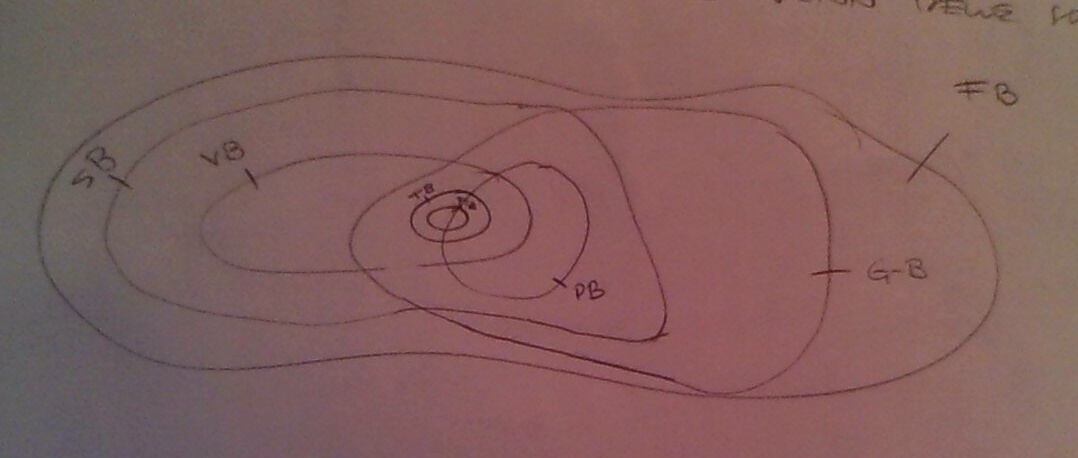
\includegraphics[width=0.5\textwidth]{Pictures/EuleroVenn_Bundles} 
  \centering
\end{figure}



\newpage
\section{Fiber Bundle}
Roughly speaking a \emph{Fiber Bundle} is a way of attach some set, the so called \emph{fibre}, on every point of another space, called \emph{Base}.
The main tool for achieving this "glueing" are the surjective function as we can guess from this observation

\begin{observation}\label{oss:BasicBundle}
$\forall$ $\pi : E \rightarrow M $ surjective function between generic set with $Dom(\pi)=E$
$$ E = \underset{p \in M}{\sqcup} \pi^{-1}(p)= \underset{p \in M}{\sqcup} E_{p}$$
\end{observation}
In this extremely simple case the sets $E_{p} =\pi^{-1}(p)$ take the role of fibers and $M$ the base. In the next section we will see that the space $E$ it's a crucial actor in the formal definition of a fiber bundle to a point that often this \emph{total space} is mistaken with the bundle itself. \cite{freed}


\subsection{Formal Definition}
\begin{remark}
In what follows all the set considered are endowed with a topological structure that is are topological space  $(X,\textrm(top)(X))$.
\end{remark}

\begin{definition}[Fiber Bundle]\label{Def:FiberBundle}
A \emph{Fiber Bundle} consists in a 4-ple $(E,B,\pi,F)$ where:
\begin{itemize}
\item[-] $E$ : topological space (called \emph{Total Space})
\item[-] $B$ : topological space (called \emph{Base Space})
\item[-] $F$ : topological space (called \emph{Typical Fiber})
\item[-] $\pi : E \rightarrow B $ continuous surjective function (called \emph{Bundle Projection})
\end{itemize}
Endowed with a \emph{Local Trivialization}:
\begin{itemize}
\item $\forall x \in E$ $\exists$ a couple $(U, \chi)$ (called \emph{local trivialization})
\begin{itemize}
\item $U$ : neighborhood of $x$
\item $\chi$ :$\pi^{-1}(U) \rightarrow U \times F$ : homeomorphism
%DaRivedere
 \footnote{surjectivity $\Rightarrow$ $\pi^{-1}(U) \neq \emptyset$.} 
 \footnote{cartesian product of topological space is a topological space with the direct product topology.}
\end{itemize}
such that: $p_1 \cdot \chi = \pi \vert_{\pi^{-1}(p)}$.

i.e: the following graph commutes:

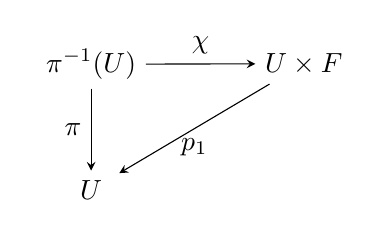
\begin{tikzpicture}
  \matrix (m) [matrix of math nodes,row sep=3em,column sep=4em,minimum width=2em] {
     \pi^{-1}(U) & U \times F \\
     U &  \\};
  \path[-stealth]
    (m-1-1) edge node [left] {$\pi$} (m-2-1)
            edge [right] node [above] {$\chi$} (m-1-2)
    (m-1-2) edge [right] node [below] {$p_{1}$} (m-2-1);;
\end{tikzpicture}

\end{itemize}
\end{definition}

\begin{figure}[h!]
  \caption{The complete fiber bundle Structure.}
  	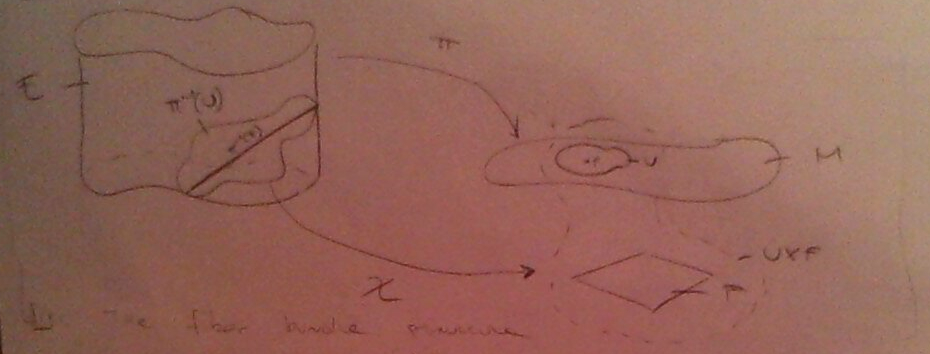
\includegraphics[width=0.5\textwidth]{Pictures/FiberBundle}
  \centering
\end{figure}

As said in the introduction, in this aggregate of objects the role of fiber attached to each point of the base space is taken by the counterimage of $\pi$. 
This deserve a proper definition:
\begin{definition}[Fiber over a point $p\in B$]
$E_{p} := \pi_{-1}(p) $
\end{definition}

Ontologically \footnote{i.e. element of one it's a different object respect the other.} we distinct between "typical fiber" and " fiber over a point" but the axiom of local trivialization assures that topologically they are the same:

\begin{lemma}
The typical fiber $F$ and the fiber upon a point are homeomorphic.
	\begin{thesis}
		$F \simeq E_{p} $ $\forall p \in B$ 
	\end{thesis}
\end{lemma}%
\begin{proof}
For each $p\in B$ is given a local trivialization $(U, \chi)$ such that $p \in U$.

Noting that $\forall $ topological space  ${p} \times A \simeq A$, follows from the definition this commutation diagram:

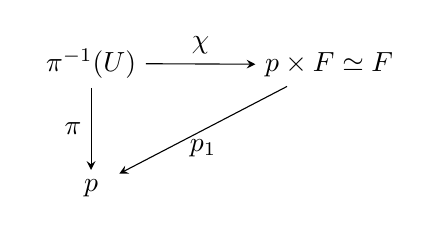
\begin{tikzpicture}
  \matrix (m) [matrix of math nodes,row sep=3em,column sep=4em,minimum width=2em] {
     \pi^{-1}(U) & {p} \times F \simeq F \\
     {p} &  \\};
  \path[-stealth]
    (m-1-1) edge node [left] {$\pi$} (m-2-1)
            edge [right] node [above] {$\chi$} (m-1-2)
    (m-1-2) edge [right] node [below] {$p_{1}$} (m-2-1);;
\end{tikzpicture}

In conclusion $\chi \vert _{E_{p}}$ realizes an homemorphism between $F$ and $E_{p}$

\end{proof}


\begin{notationfix}
It's customary to refer to the fiber bundle $(E,\pi,M ; Q)$ indicating only its total space $E$:
\begin{displaymath}
	\gls{Bundle}%E= ( E,\pi, B ; F)
\end{displaymath}

A possible, more heavy, convention is to denote the fiber bundle as a \emph{short sequence}\cite{•}
$$ Q \rightarrow E \xrightarrow{\pi} M$$
\end{notationfix}

\begin{notationfix}
	\danger(da correggere)\\
	We say that a fiber bundle $E$ is \emph{(globally) trivial} if there exists a fiber preserving diffeomorphism from $E$ to the Cartesian product $M×Q$ which is a vector space isomorphism on each fiber. 
	In practice, this corresponds to a trivialization of $E$ which is defined everywhere, to be compared with the notion of a local trivialization per Definition \ref{Def:FiberBundle}. 
\end{notationfix}

Given two bundle $E$ and $F$ on the same base $M$, it's straightforward the definition of some additional structures just performing the algebraic operations fiberwise:
\begin{definition}[Bundle Restriction]
	See  \cite{advances}.
\end{definition}
\danger : definizione ripetuta!
\begin{definition}[Cartesian Product Bundle]
	Fiber bundle $E \times_M F$ over $M$ such that :
	\begin{displaymath}
		(E \times_M F )_p = E_p \times F_p
	\end{displaymath}
	\footnote{for every point $p\in M$ , we take the tensor product of the fibers, $E_p \times E'_p$.}
\end{definition}

\begin{Warning}
	List pagg 9 \cite{primer}
\end{Warning}


\subsection{Cross Sections}
The notion of bundle is particularly interesting from the perspective of physics because provides the rigorous description of a $F-$valued field on the space $B$.

\begin{definition}[(Cross) Section]
Function $\phi : B \rightarrow E$ such that:
\begin{itemize}
\item $\phi$ continuous.
\item $\phi \cdot \pi = \textrm{Id}_{B}$ 
\end{itemize}
\end{definition}

\begin{figure}[h!]
  \caption{Section on a Bundle.}
  	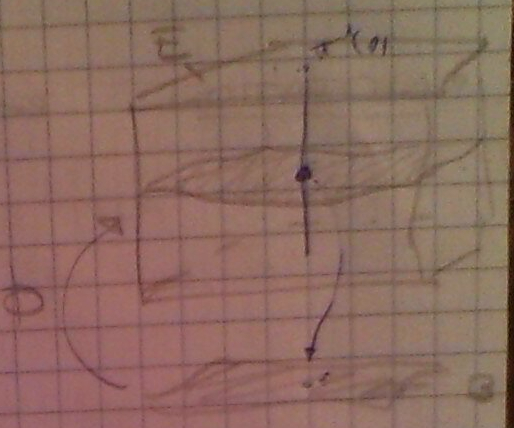
\includegraphics[width=0.5\textwidth]{TempPictures/CrossSection.jpg}
  \centering
\end{figure}

\begin{notationfix}
We refer to:
\begin{itemize}
\item \emph{Global section} $\Leftrightarrow$ $\textrm{dom}(\phi) = B$
\item \emph{Local section} $\Leftrightarrow$ $\textrm{dom}(\phi) \subset B$ \footnote{Usually the domain is an open set of B)}
\end{itemize}
\end{notationfix}

\begin{observation}
The property that essentially makes a section $\phi$ a good abstraction of a field is the following:
\begin{displaymath}
\forall p \in B \phi(p) \in \pi^{-1}
\end{displaymath}
\end{observation}

In other words:
\begin{proposition}
Local section $\{\phi \}$ are in a 1:1 correspondence with continuous function $\{ f: B \rightarrow F \} $.
\end{proposition}
\begin{proof}

%(da controllare.. su appunti ho fatto una figura)

Take $p\in B$ and $(U,\chi)$ local trivialization over $p$.

Define $f: U \rightarrow F$ as $f= p_{2} \cdot \chi \cdot \phi \vert_{U}$, where $p_{2}$ is a projection on the second element of a cartesian product space.

Then : $\chi \cdot \phi (p) = ( p, f(p) )$ (...).

\end{proof}

\begin{observation}
The preceding argument give meaning to the claim often presented in geometry books that: " cross section represent an abstract generalization to graph of functions."
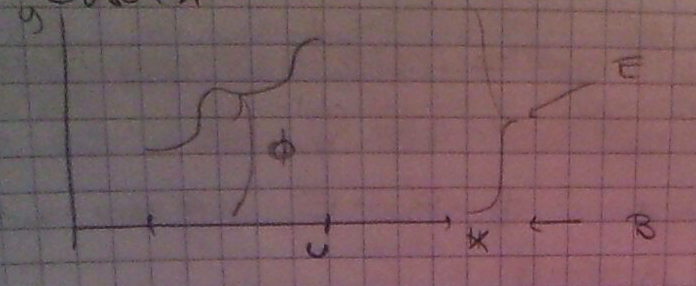
\includegraphics[width=0.5\textwidth]{TempPictures/SectionasGraph.jpg}
\end{observation}

\begin{notationfix}
The \emph{set of all section} is often denoted as:
$$\gls{Sections} $$
\end{notationfix}

\subsection{Maps between Fiber Bundles}
Consider two fiber bundle $(F,E,\pi,B)$ and $(F',E',\pi',B')$.


\begin{definition}[Bundle Morphism]
A pair of map $(\phi_{tot}, \phi_{base})$ where:
\begin{itemize}
\item[-] $\phi_{tot}:E \rightarrow E'$ continuous.
\item[-] $\phi_{base}:B \rightarrow B'$ continuous.
\end{itemize}
Such that 
\begin{equation}\label{eq:fiberbundle}
\pi' \cdot \phi_{tot} = \phi_{base} \cdot \pi
\end{equation}
, i.e the following graph commutes:
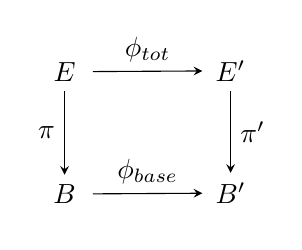
\begin{tikzpicture}
  \matrix (m) [matrix of math nodes,row sep=3em,column sep=4em,minimum width=2em] {
     E & E' \\
     B & B' \\};
  \path[-stealth]
    (m-1-1) edge node [left] {$\pi$} (m-2-1)
            edge [right] node [above] {$\phi_{tot}$} (m-1-2)
    (m-1-2) edge node [right] {$\pi'$} (m-2-2)
    (m-2-1) edge [right] node [above] {$\phi_{base}$} (m-2-2);
\end{tikzpicture}
\end{definition}

\begin{observation}
Restricting the equation \eqref{eq:fiberbundle} to act only on a specific fiber,
\begin{displaymath}
\pi' \cdot \phi_{tot} \vert_{E_{p}} = \phi_{base} \cdot \pi (E_{p}) = \phi_{base}(p) := p'
\end{displaymath}
we can see that precedent definition it's equivalent to requirement that $\phi_{tot}$ is fiber preserving:
\begin{displaymath}
\forall p \in B \qquad \phi_{tot}(E_{p}) = E_{\phi_{tot}(p)}
\end{displaymath}

Follows that to determine a bundle morphism is sufficient to provide a fiber preserving map between the total spaces. It's then customary to denote a bundle morphism with $\phi_{tot}$ only.
\end{observation}

\begin{proposition}[Fiber Bundle as a Category.]
$$ $$
	\begin{hypothesis}
			\begin{itemize}
				\item $\mathfrak{C} = $ set of all possible fiber bundle.
				\item $hom(\mathfrak{C}) = $ set of all bundle morphism.
			\end{itemize}
	\end{hypothesis}
	\begin{thesis}
		The couple ( C, hom(C)) form a concrete category.
	\end{thesis}
\end{proposition}
\begin{proof}
	Technicality (...).
\end{proof}

\begin{observation}
Note that the fiber projection of a fiber bundle is a continuous map, than an homomorphism of the topological space category (a particular one, which satisfies the axiom of local triviality).
\end{observation}

\begin{definition}[Bundle isomorphism]
A bundle morphism $(\phi_{tot}, \phi_{base})$ such that $\phi_{\cdot}$ are homeomorphism.
\end{definition}

\begin{notationfix}
It's frequent to refer at the bundle morphism between fiber bundle over the same base $( \phi_{base} = Id_{B} )$ as \emph{Fiber Preserving map}.

$\phi: E \rightarrow F $ continuous such that:
\begin{displaymath}
\phi(E_{x})= F_{x} \qquad \forall x \in M.
\end{displaymath}

i.e.:

\begin{tikzpicture}
  \matrix (m) [matrix of math nodes,row sep=3em,column sep=4em,minimum width=2em] {
     E & & F \\
       & M & \\};
  \path[-stealth]
    (m-1-1) edge node [left] {$\pi_{E}$} (m-2-2)
            edge [right] node [above] {$\phi$} (m-1-3)
    (m-1-3) edge node [right] {$\pi_{F}$} (m-2-2);
\end{tikzpicture}
\end{notationfix}

%%%%%%   Pull back Bundle   %%%%%%%%%%%%%%
\danger \href{https://en.wikipedia.org/wiki/Pullback_bundle}{Fonte wiki}
Consider a topological space $N$, a fiber bundle $E=(E,\pi,M;Q)$, and a continuous function $f: N \rightarrow M$. It's possible to induce\cite{Husemoller} a bundle structure from the manifold $M$ to $N$:
\begin{definition}[Pull-Back Bundle]
	3-ple $f^* (E) = (f^* (E) =, \pi^*,N)$ such that:
	\begin{itemize}
		\item $f^* (E) =  \big\{ (b',e) \in N \times E \quad \big\vert \; f(b') = \pi(e) \big\} $
		\item $\pi^*:f^* (E) \rightarrow N $ such that $ \pi* (b',e) = \textrm{pr}_1 (b',e)= b' $
	\end{itemize}
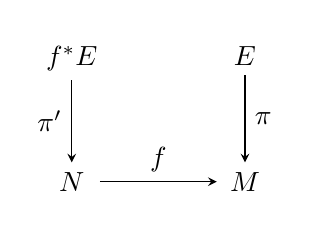
\begin{tikzpicture}
  \matrix (m) [matrix of math nodes,row sep=3em,column sep=4em,minimum width=2em] {
     f^* E & E \\
     N & M \\};
  \path[-stealth]
    (m-1-1)edge node [left] {$\pi'$} (m-2-1)
    (m-1-2) edge node [right] {$\pi$} (m-2-2)
    (m-2-1) edge [right] node [above] {$f$} (m-2-2);
\end{tikzpicture}
\end{definition}

\begin{proposition}
$f^* (E) = (f^* (E) =, \pi^*,N)$ consitute a fiber bundle of typical fiber Q.
\end{proposition}\begin{proof}
If we want to complete the fiber bundle structure we have to provide a local trivialization atlas.
$\forall ( U, \phi)$ local trivialization on $(E, \pi, M)$  consider $\psi: f^* E \rightarrow N \times Q$ such that $\psi( b',e) = \bigg( b', pr_2 \big( \phi(e)\big)\bigg)$.

Then $(f^{-1}(U),\psi)$ is a local trivialization of the pull-back bundle and the fiber of $f^*E$ over a point $b′\in B'$  is just the fiber of E over $f(b′)$.
\end{proof}

\begin{observation}
Consider this situation:

\begin{tikzpicture}
  \matrix (m) [matrix of math nodes,row sep=3em,column sep=4em,minimum width=2em] {
        & E \\
     N & M \\};
  \path[-stealth]
    (m-1-2) edge node [left] {$\pi$} (m-2-2)
    (m-2-2) edge  [bend right] node (s) [right]{$s$} (m-1-2)
    (m-2-1) edge [right] node [above] {$f$} (m-2-2);
\end{tikzpicture}
where $s \in \Gamma(\pi_M)$.
Pull-Back of Section is easily obtained as follow:
\begin{displaymath}
f^* s = s \cdot f \in \Gamma(f^* E)
\end{displaymath}

\end{observation}


%%%%%%   Mor Bundle   %%%%%%%%%%%%%%
It is also noteworthy that, given any two vector bundles $E =(E\pi,M,Q)$ and $E =(E'\pi,M',Q')$, we can construct 	naturally a third fiber bundle.
Consider $\hom(E,E')$ the set of all the fiber preserving map between the two bundles:
\begin{definition}[Bundle of morphisms]
	Fiber bundle $\hom(E,E')$ over the base space $M$ such that the fiber over a base point $p\in M$ is the infinite dimensional manifold $\hom(E_p,E'_p)$ isomorphic to $\hom(Q,Q')$.
\end{definition}
	\begin{notationfix}
	We shall write $End(F)$ for $\hom(E,E)$ and call it bundle of endomorphism, whose typical fiber is $\textrm{End}(Q)$.
	\end{notationfix}

	\begin{remark}
		If $F,F'$ are vector bundle then the fiber of  $\hom(F,F')$ over a base point $p\in M$ is $\hom(F_p,F'_p)$, which is a vector space isomorphic to the vector space $\hom(V,V')$ of linear applications from $V$ to $V'$
	\end{remark}

\subsection{Toward other type of bundle.}
Roughly speaking a fiber bundle is an agglomerate of fiber space over a different space called base. Fiber and Base could have different structure, a sort of compatibility between structure is guaranteed by the properties of $\pi$ and $\chi$.
Category theory provides the appropriate language to treat various bundle structure in a unified way.

Consider two construct $\mathbf{C}_{1}$ , $\mathbf{C}_{2}$ subcategory of $\mathbf{Top}$, concrete category of all topological spaces \footnote{Set of the object must be considered together with a cartesian product operator $\times : \textrm{obj} \times \textrm{obj} \rightarrow \textrm{obj}$.}, such that:
\begin{displaymath}
\mathbf{Top} \supseteq \mathbf{C}_{1} \subseteq \mathbf{C}_{2}
\end{displaymath}

\begin{definition}[$(\mathbf{C}_{1})-$Bundle of $(\mathbf{C}_{2})-$fiber]\label{CategoryBundle}
It's a 4-ple $(E,M,\pi,F)$ where:
\begin{itemize}
\item[-] $E, M \in \Obj(\mathbf{C}_{1})$ : (called \emph{Total Space} and \emph{Base Space})
\item[-] $F \in \Obj(\mathbf{C}_{2})$ : (called \emph{Typical Fiber})
\item[-] $\pi \in \hom(E,B) \subset \Mor(\mathbf{C}_{1})$ : (called \emph{Bundle Projection})
\end{itemize}
Such that:
\begin{itemize}
\item $\pi$ surjective.
\item $\pi^{-1} (p) \in \Obj(\mathbf{C}_{2}) \quad \forall p \in M $
\item $\forall p \in M \; \exists (\chi,U)$ (local trivialization) such that:
	\begin{itemize}
	\item $U$ is a neighbourhood of $p$
	\item $\chi \in \iso(E,U\times F)\subset \Iso(\mathbf{C}_{1})$
	\item $\chi \vert_{\pi^{-1}(p)} \in \iso(\pi^{-1}(p),\{p\}\times F)\subset \Iso(\mathbf{C}_{2}) $
	\end{itemize}
\end{itemize}
\end{definition}
the main categories of interest are the following:

\begin{tabular}{|c|c|c|c|}
\hline 
Category & Obj & Mor & Iso \\ 
\hline 
$\mathbf{Top}$ & topological spaces & continuous functions & homeomorphism \\ 
$\mathbf{Smooth}$ & smooth manifold & differentiable functions & diffeomorphism \\ 
$\mathbf{GLie}$ & Lie groups & homomorphism & group isomorphism \\ 
$\mathbf{Vec}$ & Vector spaces & linear operators & $\mathbb{GL}-$operators \\ 
\hline 
\end{tabular} 



%-_-_-_-_-_-_-_-_-_-_-_-_-_-_-_-_-_-_-_-_-_-_-_-_-_-_-_-_-_-_-_-_-_-_-_-_-_-_-_-_-_-_-_-_-_-_-_-_-_-_-_-_-_-_-_
\newpage
\section{Structure Group and transition Function}
From what we have seen seems legit to consider the local trivialization of a fiber bundle as the analogous of a a local chart on a smooth manifold.

That make sense to the idea of fiber bundle (thought as its total space) as a space which is locally a product space
\href{http://en.wikipedia.org/wiki/Vector_bundle#mediaviewer/File:Moebiusstrip.png}{link}.
( But globally may have a different structure, Not all bundle are trivial ).

However in the definition of Bundle is required the existence of at least one trivialization chart  for each point but no notion of \emph{compatibility} is explicitly required.

\subsection{The problem of \emph{Overlapping Trivialization}.}

Consider two local trivializations (with $ i = \alpha, \beta$):
\begin{displaymath}
\chi_{i} : \pi^{-1} (U_{i}) \rightarrow U_{i} \times F
\end{displaymath}
overlapping, that is $ U_{\alpha} \cap U_{\beta} \neq \emptyset$.

\begin{definition}[Transition Function (from $\alpha$ to $\beta$)]
\begin{displaymath}
g_{ \beta \alpha}: U_{\alpha} \cap U_{\beta} \rightarrow	\textrm{aut}(F)
\end{displaymath}\footnote{In the category of topological spaces $\textrm{aut}(F) $ consists of homeomorphism from $F$ to itself.}
given by
\begin{displaymath}
\chi_{\beta} \cdot \chi_{\alpha}^{-1} \big(p, \: V_{\alpha}\big) = \big( p, \: g_{ \beta \alpha} [p] (V_{\alpha}) \big )= \big(p, \:  V_{\beta} \big) \qquad \forall p \in U_{1} \cap U_{2} , \forall V_{\alpha} \in F
\end{displaymath}
\end{definition}

\begin{figure}[h!]
  \caption{Transition map between local trivialization.}
  	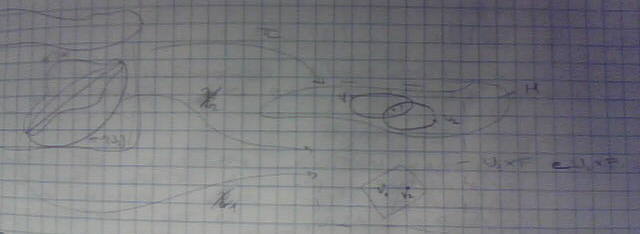
\includegraphics[width=0.5\textwidth]{TempPictures/TransitionMap.jpg}
  \centering
\end{figure}

\begin{notationfix}
It's common to refer to the transition map as the well defined homeomorphism:
\begin{displaymath}
\chi_{\beta} \cdot \chi_{\alpha}^{-1} :  ( U_{i} \cap U_{j} ) \times F   \rightarrow ( U_{i} \cap U_{j} ) \times F
\end{displaymath}
instead of the function $g_{ \beta \alpha}$ which realizes the transformation.
\end{notationfix}

In analogy with the atlas of chart on a manifold also the collection of all the local trivialization supplied to the Bundle structure takes a specific name:
\begin{definition}[Bundle (Trivialization) Atlas]
Is a collection of local trivialization which cover the entire base space: 
\begin{displaymath}
\big \{ ( U_{\alpha},\chi_{\alpha} ) \big \vert \bigcup_{\alpha} U_{\alpha} \supseteq M  \big \}
\end{displaymath}
\end{definition}

Since for each pair of overlapping map is defined a transition function, every bundle atlas carries with itself a collection of such maps:
\begin{displaymath}
\big \{ g_{ \beta \alpha} : U_{\alpha} \cap U_{\beta} \rightarrow	\textrm{aut}(F) \big \vert U_{\alpha} \cap U_{\beta} \neq \emptyset \big \}
\end{displaymath}
its cardinality is determined by the number of overlapping open set in the atlas.



\begin{proposition}
The transition maps relating to a specific atlas always meet the following properties:
\begin{equation}\label{cocycle a}
g_{ \alpha \alpha} (p) = \mathds{1}_{F}  \qquad \forall p \in U_{\alpha}
\end{equation}
\begin{equation}\label{cocycle b}
g_{ \beta \alpha} (p) = g_{ \alpha \beta}^{-1} (p)  \qquad \forall p \in U_{\alpha} \cap U_{\beta}
\end{equation}
\begin{equation}\label{cocycle c}
g_{ \beta \gamma} (p) g_{ \gamma \alpha} (p)  = g_{  \beta \alpha} (p)  \qquad \forall p \in U_{\alpha} \cap U_{\beta} \cap U_{\gamma} \footnote{\emph{cocycle condition}}
\end{equation}
\end{proposition}
\begin{proof}
\begin{itemize}
\item \eqref{cocycle a} follows from the composition rule: $$\chi_{\alpha} \chi_{\alpha}^{-1} = \mathds{1}_{U_{\alpha}\times F} $$

\item \eqref{cocycle b} follows from: $$\big ( \chi_{\alpha} \cdot \chi_{\beta}^{-1} \big)^{-1} = \chi_{\beta} \cdot \chi_{\alpha}^{-1}$$

\item \eqref{cocycle c} follows from: 
\begin{displaymath}
\big( p , g_{\beta \alpha}(p) V \big) = \big[  \chi_{\beta} \cdot \chi_{\alpha}^{-1}  \big] (p, V) =  \big[  \chi_{\beta} \cdot \chi_{\gamma}^{-1}  \big] \big[  \chi_{\gamma} \cdot \chi_{\alpha}^{-1}  \big] (p, V) = \big( p , g_{ \beta \gamma} (p) g_{ \gamma \alpha} (p)  V \big) 
\end{displaymath}

\end{itemize}
\end{proof}

\subsection{Structure Group}	
From the definition is clear that the transformation maps are valued in a  group (the group of automorphism $\textrm{aut}(F) $) but in general the set $\{ g_{\alpha \beta}[p] \}$ for a fixed $p$ don't form a subgroup \footnote{Or , equivalently, the map $\{ g_{\alpha \beta} \}$ is not the action of some group.}. 

\begin{example}
Being a group would means  that fixed four overlapping trivialization$ \alpha, \beta, \gamma, \delta$ must exists another couple of trivialization $\theta , \eta$ such that:
\begin{displaymath}
g_{\alpha \beta } \cdot g_{\gamma \delta} = g_{\theta \eta}
\end{displaymath}
obviusly there's no natural way of construct such composition from the cocycle condition only.
\end{example}

For this reason, the following definition arise spontaneously:
\begin{definition}[G-Atlas]
It's a trivialization atlas $\{ (U_i , \chi_i ) \}$ such that the corresponding transition maps constitutes a group left-action of the abstact group $G$ on the fiber space $F$.
\end{definition}

\begin{notationfix}
It's common to use the following names when referring to a G-structered fiber bundle:
\begin{itemize}
\item \emph{G-Bundle} : fiber bundle rigged with a G-atlas of trivialization.
\item \emph{Structure group} : the abstract group $G$ whose actions realize the transition maps.
\end{itemize}

\end{notationfix}

The choose of such solemn name for the structure group is justified by the following theorem:
\begin{theorem}\cite{freed}
Fixing a typical fiber $F$, a base space $M$ and a G-action $g_{\alpha \beta}$ which map the transition function is sufficient to determine the G-Bundle $(F,E,\pi,M,G )$.
	\begin{hypothesis}
			\begin{enumerate}
				\item $M,F$ topological spaces. 
				\item $\{U_{\alpha}\}_{\alpha \in I} $ open cover of $M$.
				\item is given a family  $\{ g_{\alpha \beta} : U_{\alpha} \cap U_{\beta} \rightarrow \textrm{aut}(F) \}$ such that:
					\begin{itemize}
					\item $ g_{\alpha \beta} : (p,f) \mapsto g_{\alpha \beta}(f) $ is an homeomorphism.
					\item $g_{ \alpha \alpha} (p) = \mathds{1}_{F}  \qquad \forall p \in U_{\alpha}$
					\item $g_{ \beta \alpha} (p) \cdot g_{ \alpha \beta} (p) = \mathds{1}_{F}  \qquad \forall p \in U_{\alpha} \cap U_{\beta}$
					\item $g_{ \beta \gamma} (p) \cdot g_{ \gamma \alpha} (p)  \cdot g_{  \alpha  \beta} (p) = \mathds{1}_{F} \qquad \forall p \in U_{\alpha} \cap U_{\beta} \cap U_{\gamma}$
					\end{itemize}
			\end{enumerate}
	\end{hypothesis}
	
	\begin{thesis}
			\begin{enumerate}
				\item The quotient space$ E = \dfrac{\bigcup_{\alpha \in I} (U_{\alpha}\times F)}{\sim}$ with : 
				$$ \big( p_{\alpha}, f \big) \sim \big( p_{\beta}, g_{\beta,\alpha}(f) \big) \qquad \forall p_{\alpha}= p_{\beta} \in U_{\alpha} \cap U_{\beta} \; \forall f\in F  $$
				endowed with the quotient topology is a topological space.
				\item The projections on the first argument $p_1 :  U_{\alpha} \times F \rightarrow U_{\alpha}$ fitted together defines a good bundle projection $\pi :E \rightarrow M$, i.e.:
					\begin{itemize}
					\item $\pi$ injective
					\item $\forall p \; \pi^{-1}(p) \textrm{homemorphic to } F$
					\end{itemize}
			\end{enumerate}
	\end{thesis}

\end{theorem}
\begin{proof}
See theorem \ref{Teo: Reconstruction Vector Bundle 1} for the demostration in a rather simpler case.
\end{proof}



\subsection{A glance on Principal Bundle}
Imposing a further prescription on the properties of a G-structure  on a G-Fiber Bundle we can identify a particular structure often used in mathematical physics.

\begin{definition}[Principal Bundle]
Is a G-bundle such that the transition maps $t_{\alpha \beta}$ as an action of the group $G$ is:
\begin{itemize}
\item[-] \emph{free} : $ \forall g \in G\setminus \{\mathds{1} \} \quad : \quad t_{[g]} \cdot s \neq s \quad \forall s \in F$
\item[-] \emph{transitive} : $\forall x,y \in F , \exists g \in G \setminus \{\mathds{1} \}$ such that : $ t_{[g]} x = y$.
\end{itemize}
\end{definition}

\begin{observation}
A such action permit a complete identification of $F$ with the group $G$.

For this reason is common place in the literature to present this further structured bundles as fiber bundle where the typical fiber $F$ is endowed with a Lie group structure and such that the local trivialization functions are Lie group isomorphism when restricted on a fiber.
\end{observation}




%-_-_-_-_-_-_-_-_-_-_-_-_-_-_-_-_-_-_-_-_-_-_-_-_-_-_-_-_-_-_-_-_-_-_-_-_-_-_-_-_-_-_-_-_-_-_-_-_-_-_-_-_-_-_-_
\newpage
\section{Smooth Bundle}
In the context of mathematical physics is more frequent referring to smooth fiber bundle instead of only topological ones.
From \ref{CategoryBundle} follows the following definition:

\begin{definition}[Smooth Fiber Bundle]
Is  a fiber bundle $(F,E, \pi, M )$ such that:
\begin{itemize}
\item $E,F,M$ are not only topological but smooth manifold.
\item $\pi$ is a smooth surjective function.
\item $\chi_{\alpha} $ is a diffeomorphism $\forall \alpha$.
\end{itemize}
\end{definition}

Since all differentiable manifolds are, in first instance, topological spaces all the statement above remain valid with the exception of consider all function \emph{differentiable} instead of \emph{continuous} only.
(e.g. in this framework the section are also differentiable, some texts use the symbol $\Gamma^{\infty} (\pi_M)$ to stress this fact.) 
\\
The few more peculiarity in considering this additional smooth structure on the spaces constituting the bundles essentially come from the presence of the local charts and the tangent spaces.

\subsection{Relation between local charts and local trivializations.}
When a smooth fiber bundle $(F,E,\pi,M)$ is considered, in addition to the typical functions of the bundle $(\pi, \chi_{\alpha})$ are to be taken in account all the collection of local chart for the three manifold : $(U_{\alpha_k}, \phi_{\alpha_k})_{k = E,M,F}$.
The context require to not confuse the chart with the trivialization even if there is a relationship between them:

\begin{proposition}
Atlas on $M$ and $F$ induce an atlas on $E$ through the local trivialization.
\end{proposition}
\begin{proof}
Consider $(U, \phi_{M})$ and $(V, \phi_{F})$ local charts on $M$ and $F$ respectively.
\\
Every local trivialization $(U_{\alpha}, \chi_{\alpha})$ such that $U_{\alpha} \supseteq U$ is a diffeomorphism, 
\\
therefore $\chi^{-1}:(U \times V) \mapsto W \in \mathcal{T}(E)$ maps open set in open set, thus 
\begin{displaymath}
\big( \chi^{-1} ( U \times	V), (\phi_{M} \times \phi_{F}) \cdot \chi \big)
\end{displaymath}
is a local chart on the manifold $E$.
\\
Since such local trivialization exist for all point in $M$ with this process is possible to map each fiber and then consitute a whole atlas on E.
\end{proof}

\begin{proposition}[vice versa]
An atlas on $E$ induce an atlas on $M$ and $F$ through the local trivialization.
\end{proposition}
\begin{proof}
Consider $(W, \phi_{E})$ local chart on $E$ and a local trivialization $(U_{\alpha}, \chi_{\alpha})$ on $M$.
\\
Take an open set $U' \subset U_{\alpha}$ in $M$ , $\pi$ is continuous then $W' = W \cap \pi_{-1}(U')$ is an open set in $E$. Moreover $V'= p_{2} \cdot \chi_{\alpha} ( W')$ is an open set in $F$.
\\ 
In conclusion $\phi_{E} \cdot \chi_{\alpha}^{-1}$ constitute a chart on $U' \times V'$ and, by projection on components of the cartesian product, on the manifold $M$ and $F$.
\end{proof}
Furthermore could be useful defining a patch on $M$ which map the base spaces and trivializes the bundle in the same time:
\begin{definition}[Local chart (of M) trivializing (E)]
Triple $(U, \phi, \chi)$ such that:
\begin{itemize}
\item $U$ open set in $M$.
\item $\phi: U \rightarrow \mathbb{R}^{\textrm{dim}(M)}$ diffeomorphism.
\item $\chi: \pi^{-1}(U) \rightarrow U \times F $ trivialization. 
\end{itemize}
\end{definition}

\begin{observation}
At this point we can see a source of confusion that comes from the identification of the whole fiber bundle $(F,E,\pi,M)$ with the total space $E$ only:
$$ \textrm{Bundle Atlas} \neq \textrm{Atlas of charts on the manifold E}$$
\end{observation}

That suggests to aggregate the two concepts in an unique definition:
\begin{definition}[Trivializing Atlas of charts]\label{Def: TrivializatingAtlas}
Collection of local charts of $M$ which trivilizes $E$ such that:
\begin{displaymath}
\big\{ (U_{\alpha}, \phi_{\alpha}, \chi_{\alpha} \vert \bigcup_{\alpha} U_{\alpha} \supseteq M   \big\}
\end{displaymath}
\end{definition}

\begin{notationfix}
Is customary to consider such atlas of trivializing charts as the proper \emph{bundle atlas} of a smooth bundle.
\end{notationfix}

\subsection{Lifting objects from the base space to the complete space}
There're basically two idea under the concept of \emph{lift} and \emph{drop} in a smooth fiber bundle.
\begin{itemize}
	\item $E$ and $M$ are smooth manifold, then it's perfectly legit to consider the tangent spaces on both of them.
	\item $\pi$ is a smooth map, then are well defined the notion of pull-back and push-forward (through the differential $\textrm{d}\pi$. 
\end{itemize}

\emph{Drop} and \emph{Lift} are only two different name, introduced for this context, for the mapping trough the differential of the projection function.
\\
Consider a parametrized curve $ \gamma: \mathbb{R}\rightarrow E$ on the total space:
\begin{definition}[Drop of curves]
Parametrized curve $\gamma^{D}: \mathbb{R}\rightarrow E$, such that:
\begin{displaymath}
\gamma^{D} = \pi \cdot \gamma
\end{displaymath}
\end{definition}
Regarding the tangent vectors as velocity vectors of equivalence classes of curves follows easly the next definition:
\begin{definition}[Drop of vectors]
\begin{displaymath}
\forall v \in T_{e_{p}}E \quad v^D := \textrm{d}\pi \cdot v = V_{\ast} \in T_{p}M
\end{displaymath}
where $e_p$ is a point of $E$ in the fiber over $p$.
\end{definition}

\begin{definition}[Lift of 1-forms]
\begin{displaymath}
\forall \alpha \in T_p^*M \quad \alpha^L := \alpha^{*} \in T_{e_{p}}^*E
\end{displaymath}
where $e_p$ is a point of $E$ in the fiber over $p$.
\end{definition}

\begin{figure}[h!]
  \caption{Lift Drop1.}
  	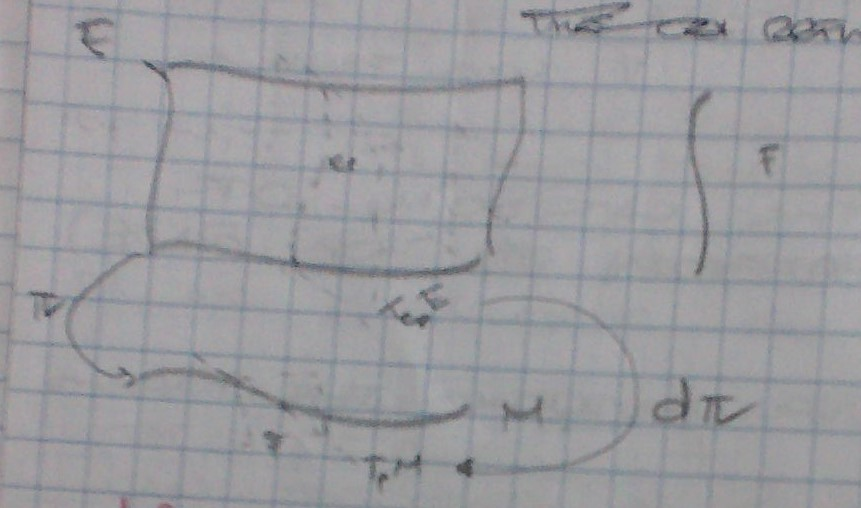
\includegraphics[width=0.5\textwidth]{TempPictures/LiftDrop1.jpg}
  \centering
\end{figure}

\begin{observation}
The former operation are naturally implemented by the presence of the special smooth function $\pi$, on the contrary their inverse are not natural ($\pi$ is not invertible) and require some additional structure like the choose of a cross-section.
\end{observation}

\subsection{Decomposition in vertical and horizontal tangent space.}
On the total space of a bundle is naturally identified a special class of curves:
\begin{definition}[locally vertical curves]
\begin{displaymath}
\gamma : \mathbb{R}\rightarrow E \textrm{ such that: } \exists U \subseteq \mathbb{R} : \pi(\gamma) \vert_U =p
\end{displaymath}
i.e. are curves of which at least a portion of them lies entirely on a fiber.
\end{definition}

\begin{figure}[h!]
  \caption{Locally vertical curve.}
  	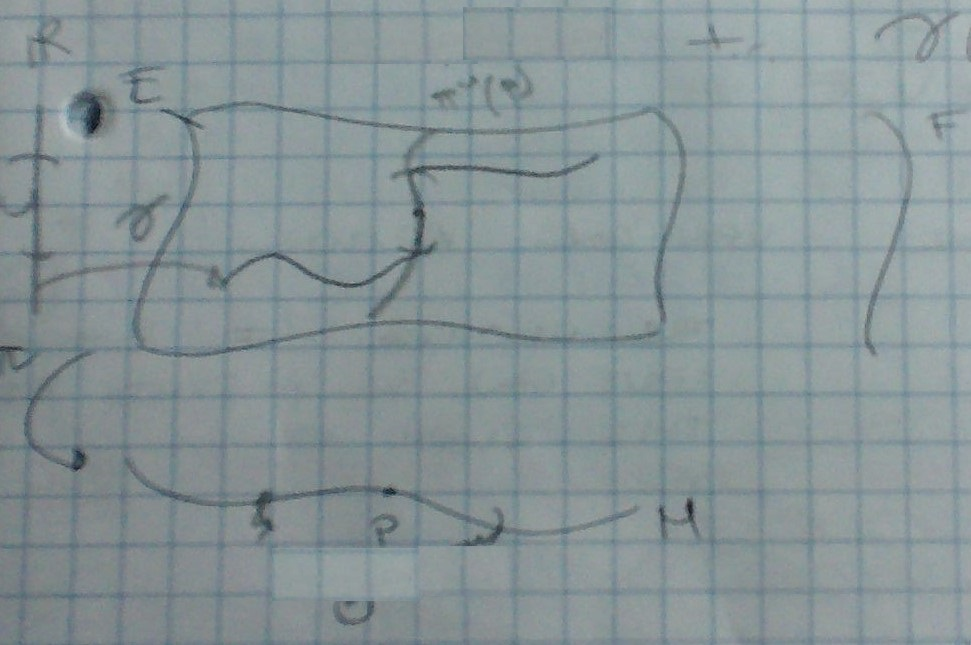
\includegraphics[width=0.5\textwidth]{TempPictures/LocalVerticalCurves.jpg}
  \centering
\end{figure}

Follows the concept of vertical vectors:
\begin{definition}[Vertical Vector]
$v \in T_e E$ is vertical if $\big( \textrm{d}\pi \big) (v) =0$
\end{definition}

\begin{observation}
The drop of a vertical curve can be seen as the motion of a particle which remain still in p for an interval $U$ of time in his parameter space.

  	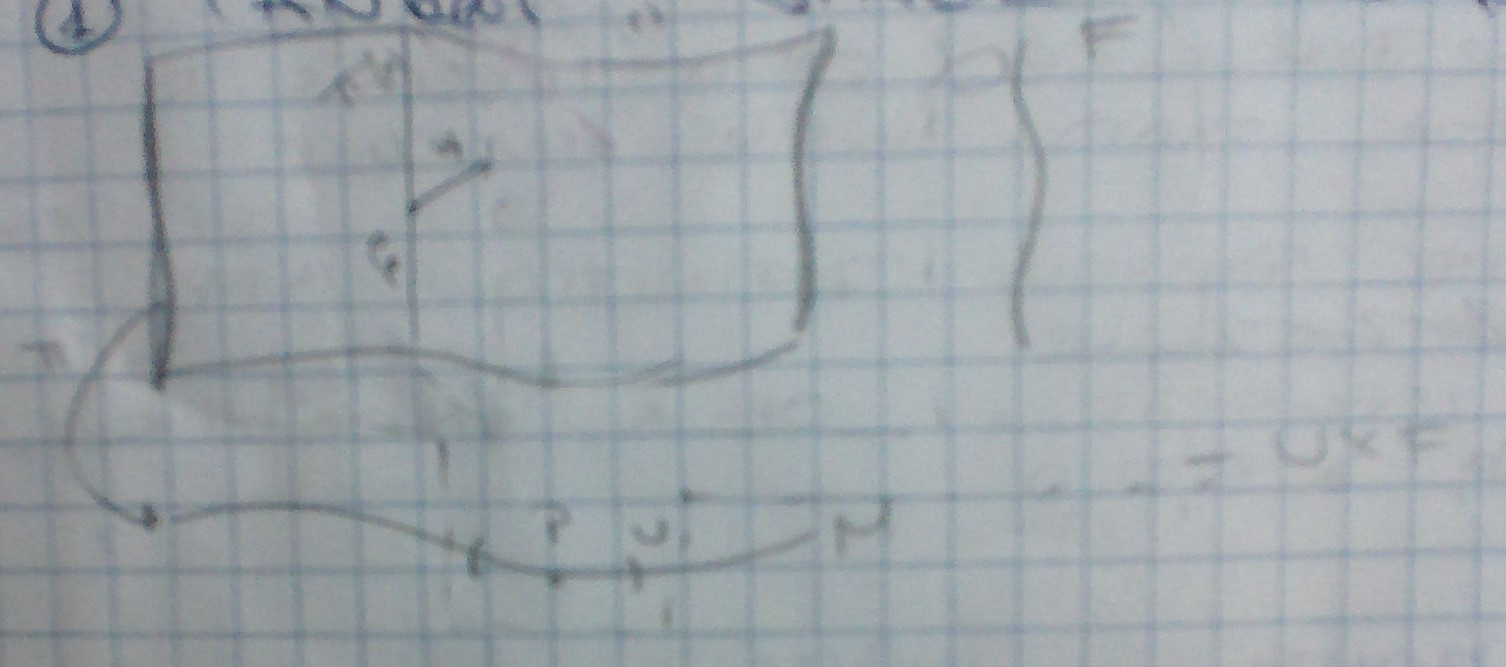
\includegraphics[width=0.5\textwidth]{TempPictures/DropofVerticalCurve.jpg}
  	Take $M,N$ manifold and  $\phi:M \rightarrow N$ smooth. \\ Be $\textrm{d}\phi_p(\dot{\gamma}) = 0 \; \forall p \in \gamma(U)$.\\ Then $\gamma' = \phi \cdot \gamma$ is the trajectory of a point which remain still for $t \in U \subset \mathbb{R}$.

\end{observation}

\begin{definition}[Vertical Tangent SubSpace]
\begin{displaymath}
V_e E = \textrm{ker}( \textrm{d}\pi) \; \subset T_e E
\end{displaymath}
\end{definition}

\begin{observation}
$V_e E$ coincides with the tangent space to the submanifold $\pi^{-1}(p) \subset E$ in the point $e_p$.
\end{observation}


\begin{definition}[horizontal Tangent SubSpace]
Complementary subspace\footnote{one out of many.} $H_e E \subset T_e E$.
i.e. such that $T_e E = H_e E \oplus V_e E$
\end{definition}

\begin{observation}
Where the vertical subspace is univocally determined by $\pi$ his complementary , the horizontal subspace, is not unique in general.
\end{observation}
The choice of such names can be argued from figure \ref{fig:VerHorSubspaces}.
\begin{figure}[h!]
  \caption{Comparison between drop of vertical and general curve (or vectors).}\label{fig:VerHorSubspaces}
  	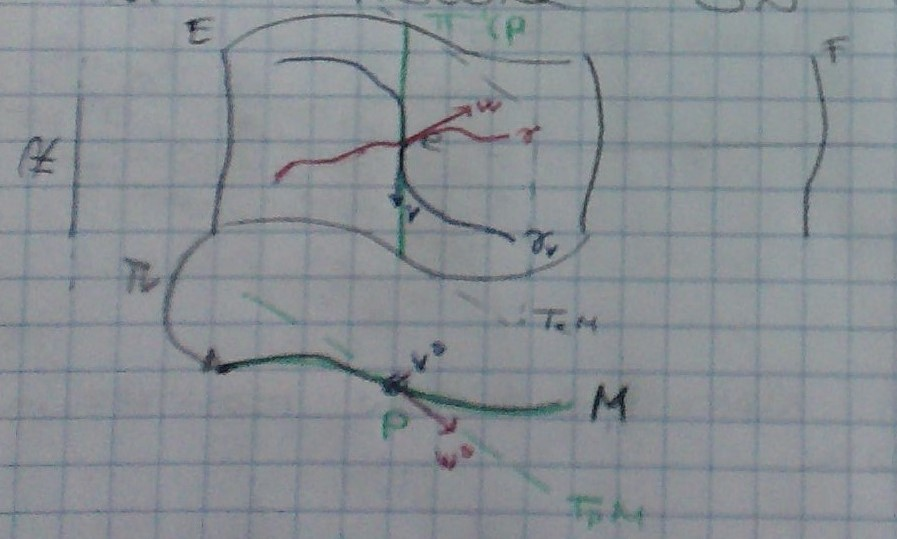
\includegraphics[width=0.5\textwidth]{TempPictures/VerHorSubspaces.jpg}
  \centering
\end{figure}

\begin{observation}[First take on the concept of Fiber Connection]
We have just seen that the concept of \emph{vertical component} of a tangent vector is coupled with the drop of vectors and is univocally determined by the fiber projection $\pi$ present on the bundle.
\\
This is not true for the opposite concept of \emph{horizontal component}. In general there is not a natural way of selecting a fixed complementary space but additional structure is needed (e.g. a condition of orthogonality provided by a riemmanian metric).
\\
The specification of an horizontal subspace for every point in $E$ is an additional structure called \emph{Fiber Bundle Connection}
\end{observation}


	


%-_-_-_-_-_-_-_-_-_-_-_-_-_-_-_-_-_-_-_-_-_-_-_-_-_-_-_-_-_-_-_-_-_-_-_-_-_-_-_-_-_-_-_-_-_-_-_-_-_-_-_-_-_-_-_
\newpage
\section{Vector Bundle}
Specializing further the smooth fiber bundle imposing the linear space structure leads us to define the \emph{vector bundle}.

\begin{definition}[Vector Bundle]
Is  a smooth fiber bundle $(V,E, \pi, M )$ such that:
\begin{itemize}
\item $V$, typical fiber space, is a vector space.
\item All the trivialization $\chi_{\alpha} $ are diffeomorphism such that:
\begin{displaymath}
	\chi_{\alpha}\vert_{\pi^{-1}(p)} \in \mathbb{GL}(n, \mathbb{R})
\end{displaymath}
\end{itemize}
\end{definition}

\begin{observation}
It's frequent in literature to present the vector bundle as a smooth bundle with typical fiber $\mathbb{R}^n$.
\\
If we just consider finite dimensional fiber vector space the difference is totally irrelevant in virtue of the well known natural\footnote{In the sense that is not dependent by the chosen basis } isomorphism $V\simeq \mathbb{R}^n$ of vector decomposition in components on a base.
\end{observation}
To encompass this two slightly different point of view we make a little revision of the definition of \emph{trivialization} in the context of vector bundle:

\begin{definition}[Local chart (of M) trivializing (E)]
Triple $(U, \phi, \chi)$\footnote{It's a standard trivializing chart with the extra feature of defining implicitly a decomposition of $V$ on a basis.} such that:
\begin{itemize}
\item $U$ open set in $M$.
\item $\phi: U \rightarrow \mathbb{R}^{\textrm{dim}(M)}$ diffeomorphism.
\item $\chi: \pi^{-1}(U) \rightarrow U \times \mathbb{R}^n $ trivialization chart.
\end{itemize} 
\end{definition}

\begin{observation}
If we consider a whole atlas of such chart will follows that the transition maps will be $\mathbb{GL}(n, \mathbb{R})$ valued, in other words the $g_{\alpha \beta}$ will be change of basis matrix.
\end{observation}

\subsection{Construction of a Vector Bundle.}
The next theorem represent a criteria to establish when a collection of isomorphic vector spaces constitutes a vector bundles.
\begin{theorem}\label{Teo: Reconstruction Vector Bundle 1}
Given an "almost"\footnote{Similar to the case presented in observation \ref{oss:BasicBundle}.} vector bundle it's sufficient to provide a collection of transition functions to complete the structure.
	\begin{hypothesis}
			\begin{enumerate}
				\item $M$ = smooth manifold
					\\ $E$ = simple set (\underline{not} a manifold)
					\\ $\pi: E \rightarrow M$ = surjective function (\underline{not} smooth)
				\item Endowed with an "almost" open trivialization atlas:
					\\ $\mathcal{A}= \big\{ (U_{\alpha}, \chi_{\alpha}) \big \}$ such that
						\begin{itemize}
						\item $\{ U_{\alpha} \}$ it's an open cover of $M$.
						\item $\chi_{\alpha} : \pi^{-1}(U_{\alpha}) \rightarrow U_{\alpha} \times \mathbb{R}^n$ bijective (\underline{not} diffeomorphism) and $p_1 \cdot \chi_{\alpha} = \pi$.
						\end{itemize}
				\item Is provided a chart atlas $(U_{\alpha}, \phi_{\alpha})$ on the precedent open cover together with all the \emph{transition map} $g_{\alpha \beta}$, i.e:
				\begin{displaymath}
				\forall (\alpha, \beta) : U_{\alpha} \cap U_{\beta} \neq \emptyset \; \exists g_{\alpha \beta} : U_{\alpha} \cap U_{\beta} \rightarrow \mathbb{GL}(n, \mathbb{R}) \; \textrm{diffeomorphism}
				\end{displaymath}
				such that:
				\begin{displaymath}
					\chi_{\alpha} \cdot \chi_{\beta}^{-1} (p , \vec{v}) = ( p, g_{\alpha \beta}(p) \vec{v} ) 	
				\end{displaymath}					
			\end{enumerate}
	\end{hypothesis}
	
	\begin{thesis}
		$E$ admit an unique vector bundle structure in which $\chi_{\alpha}$ are local trivialization.
	\end{thesis}
\end{theorem}

The hypothesized structure lacks the following properties in order to form a vector bundle:
\begin{itemize}
\item[a)] The fiber upon a point has to be isomorphic to the typical fiber, i.e. $ E_p \simeq \mathbb{R}^n \quad \forall p$.

\item[b)] $E$ has to be a smooth manifold.

\item[c)] $\chi$ has to be a diffeomorphism

\item[d)] $\pi$ has to be differentiable.
\end{itemize}

\begin{proof}
\begin{itemize}
\item[a)]  Using Hp.2 is possible to associates $\forall V \in E$ $\vec{V}\in \mathbb{R}^n$ biunivocally:
	\begin{displaymath}
	\chi_\alpha \vert_{E_p}: V_p \in E_p \leftrightarrow \vec{V} \in \{p\} \times \mathbb{R}^n \simeq 	\mathbb{R}^n 
	\end{displaymath}
Then endow $E_p$ with a natural vector bundle structure:
	\begin{displaymath}
	u_1 + \lambda u_2 = \chi_\alpha^{-1} \big( p, \vec{u_1} + \lambda \vec{u_2} \qquad \forall u_1,u_2 \in E_p \; \forall \lambda \in \mathbb{R}
	\end{displaymath}
\vspace{5mm}
In other words all local trivialization containing p induce a vector space structure, this is is well defined if the linear composition defined through $\chi_\alpha$ is the same as the structure defined through $\chi_\beta$ $\forall p \in U_\alpha \cap U_\beta$.
\\
Take $u \in E_p$ and define $\vec{v},\vec{u}$ such that $\chi_\alpha (u) = \big(p, \vec{v} \big)$ and $\chi_\beta (u) = \big(p, \vec{w} \big)$.
\\
By Hp.3 $(p, \vec{V_\alpha})= \chi_\alpha \circ \chi_\beta^{-1}(p, \vec{V_\beta}) = (p, [g_{\alpha \beta}](p)\vec{V_\beta})$
So the good definition is assured by:
	\begin{eqnarray}
		(u_1 + \lambda u_2)^{(\alpha)} = \chi_\alpha^{-1} (p, \vec{v_1} + \lambda \vec{v_2} =
		\chi_\alpha^{-1} (p, g_{\alpha \beta}\vec{w_1} + \lambda g_{\alpha \beta}\vec{w_2} =\\=
		\chi_\alpha^{-1} (p, g_{\alpha \beta}(\vec{w_1} + \lambda \vec{w_2} =
		\cancel{\chi_\alpha^{-1} \circ\chi_\alpha }\circ \chi_\beta^{-1}(p, \vec{w_1} + \lambda \vec{w_2}= (u_1 + \lambda u_2)^{(\beta)}
	\end{eqnarray}

\item[b)] It's possible to endow $E$ with an atlas of compatible charts.
	\\
	$\{\pi^{-1}(A) \vert A \in \textrm{top}(M) \}$ constitutes a topology on $E$.
	\\
	Surjectivity of $pi$ $\Rightarrow$ $\{\pi^{-1}(U_\alpha) =\tilde{U_\alpha} \}$ it's an open cover of $E$.
	\\
	$\tilde{\chi_\alpha}: \pi^{-1}(U_\alpha) \rightarrow \mathbb{R}^{\textrm{dim}(M)}\times \mathbb{R}^n$ such that $tilde{\chi_\alpha} = ( \phi_\alpha \times \mathbb{1} ) \circ \chi_\alpha$ consitutes a chart on $E$ $\forall \phi_\alpha$ chart on  $M$.
	\\
	Transition chart are smooth because composition of two smooth function:
	\begin{displaymath}
	\tilde{\chi_\alpha}\circ \tilde{\chi_\beta^{-1}} = (\phi_\alpha \circ \phi_\beta^{-1}, g_{\alpha \beta} )
	=(\phi_\alpha \circ \phi_\beta^{-1}) \times ( g_{\alpha \beta} )
	\end{displaymath}
	\vspace{5mm}
	Then $\tilde{\mathcal{A}} = \{( \tilde{U_\alpha}, \tilde{\chi_\alpha} ) \}$ constitutes an atlas of $C^\infty-$compatible charts.

\item[c)] $\chi_\alpha: \pi^{-1}(U_\alpha) \rightarrow U_\alpha \times \mathbb{R}^n$ it's smooth if $(\phi_\alpha \times \mathbb{1}) \circ \chi_\alpha \circ \tilde{\chi_\alpha}^{-1}: \mathbb{R}^{m+n}\rightarrow \mathbb{R}^{m+n}$ is also smooth , that's guaranteed by its definition:
	\begin{displaymath}
	(\phi_\alpha \times \mathbb{1}) \circ \chi_\alpha \circ \tilde{\chi_\alpha}^{-1}= (\phi_\alpha \times \mathbb{1}) \circ \chi_\alpha \circ \big( (\phi_\alpha \times \mathbb{1}) \circ \chi_\alpha \big)^{-1} = \mathbb{1}
	\end{displaymath}	 
\item[d)] $\pi : \pi^{-1}(U_\alpha) \rightarrow U_\alpha $ is smooth if $\phi_\alpha \circ \pi \circ \tilde{\chi_\alpha}^{-1}$ is also smooth, that's guaranteed by Hp.2:
	\begin{displaymath}
		\phi_\alpha \circ \pi \circ \tilde{\chi_\alpha}^{-1} =
		\phi_\alpha \circ \pi \circ \chi_{\alpha}^{-1} \circ (\phi_\alpha \times \mathbb{1})^{-1} =
		\phi_\alpha \circ p_1 \circ ( \phi_\alpha^{-1} \times \mathbb{1} ) \mathbb{1}
	\end{displaymath}
\end{itemize}


\end{proof}


\begin{theorem}\label{Teo: Reconstruction Vector Bundle 2}
It's possible to reconstruct a vector bundle only from the transition maps.
	\begin{hypothesis}
			\begin{enumerate}
				\item Be $M$ a smooth manifold and $\mathcal{A}= \{(U_{\alpha}, \phi_{\alpha} \}$ atlas of local charts.
				\item $\forall$ couple $ U_{\alpha},U_{\beta} \in \mathcal{A}$ is given a map $g_{\alpha \beta} : U_{\alpha} \cap U_{\beta} \rightarrow \mathbb{GL}(n, \mathbb{R})$ \\such that:
				\begin{enumerate}[(a)]
					\item $g_{ \alpha \alpha} (p) = \mathds{1}_{F}  \qquad \forall p \in U_{\alpha}$
					\item $g_{ \beta \alpha} (p) = g_{ \alpha \beta}^{-1} (p)  \qquad \forall p \in U_{\alpha} \cap U_{\beta}$
					\item $g_{ \beta \gamma} (p) g_{ \gamma \alpha} (p)  = g_{  \beta \alpha} (p)  \qquad \forall p \in U_{\alpha} \cap U_{\beta} \cap U_{\gamma}	$			
				\end{enumerate}
			\end{enumerate}
	\end{hypothesis}
	
	\begin{thesis}
		\begin{enumerate}
		\item It's defined a vector bundle on base space $M$ with $g_{\alpha \beta}$ transition maps.
		\item Such bundle is unique up to isomorphisms.
		\end{enumerate}
	\end{thesis}
\end{theorem}
\begin{proof}
	See for example Abate\cite{Abate}, page 137.
\end{proof}

We can state the content of previous demostration as follow:
\begin{corollary}
%(questa effettivamente è solo una ripetizione del teorema precedente!)
	\begin{hypothesis}
		Provided the hypothesis of theorem \ref{Teo: Reconstruction Vector Bundle}.
	\end{hypothesis}
	\begin{thesis}
	\begin{enumerate}
	\item $E=\frac{\underset{\alpha \in \mathcal{A}}{\sqcup}U_{\alpha}\times V}{\sim}$ \\ with $(x,v) \sim (y,w) \Leftrightarrow (x=y) \wedge w= g_{\beta \alpha}(x)v$ \\where $ x\in U_{\alpha};\: y \in U_{\beta};\: v,w \in V$
	\\ consitutes a smooth manifold.
	\item Taken $\pi: E \rightarrow M$ such that $\pi(x,v) =x$ \\ then $(V,E,\pi,M)$ consitute a vector bundle.
	\end{enumerate}
	\end{thesis}
\end{corollary}

\subsection{Vector fields and References.}
There are few more feature than the abstract section:
\begin{enumerate}
	\item $\Gamma(\pi_M)$ of a vector bundle inherit the linear properties from $F$ defining sum and product by a 	scalar pointwise:
		\begin{displaymath}
			\forall s_i \in \Gamma(\pi_M) \qquad
            	   \begin{array}{ll}
                  \big( s_1 + s_2 \big) (p) = \big( s_1 \big) (p) + \big( s_2 \big) (p) \\
                  \big( \lambda s_1 \big) (p) = \big( \lambda s_1 (p) \big)
                \end{array}
		\end{displaymath}
	\item There's a special cross-section called \emph{null section}:
		\begin{displaymath}
			O_{E} \in \Gamma(\pi_M) \quad \textrm{such that:} \quad O_{E}(p) = 0\big\vert_{\small E_p} \forall p\in M
		\end{displaymath}			
	\item It's possible to extend the concept of basis from $F$ to $\Gamma(M)$.
\end{enumerate}

\subsubsection{Local reference.}
Consider a vector bundle $(F,E,\pi,E)$ of finite dimension $dim(F)= f < \infty$

\begin{definition}[Local reference]
r-ple $\{ \sigma_1, \ldots, \sigma_r \} $ of sections $\sigma_i \in \Gamma(U)$ on  $U \subset E$ open set, 
such that $\{ \sigma_1(p), \ldots, \sigma_r(p) \}$ constitues a  basis in $E_p \forall p \in U$.
\end{definition}

\begin{proposition}
Giving a local reference is equivalent to give a bundle atlas
\end{proposition}
\begin{proof}
\begin{itemize}
\item[$\Leftarrow$] Giving a reference through a local trivialization is rather simple.
	\\ Chosen a basis $\{ e_j \}$ in $F$,
	\begin{displaymath}
		\Gamma(U) \ni \sigma_j (p) = \chi^{-1}(p, e_j)
	\end{displaymath}	 
	is a local reference.

\item[$\Rightarrow$]
	Vice versa $\forall $ local reference $\{ \sigma_1, \ldots, \sigma_r \} $ on $U$ we can define:
	\begin{displaymath}
	\xi: U \times \mathbb{R}^r \rightarrow \pi^{-1}(U) \quad \textrm{such that:} \; \xi(p,\vec{w}) = w^i \sigma_i(p) 
	\end{displaymath}
	\begin{itemize}
	\item[-] $\xi$ is bijective, follows from the definition of reference.
	\item[-] $\xi$ is smooth from linearity in $w^i$ variable and smoothness of section in $p$ variable. 
	\item[-] follows from the definition that $\chi := \xi^{-1}$ trivializes E.
	\item[-] Smoothness of $\chi$ follows from the following argument:
		\\ Consider a second local trivialization $\tilde{\chi}$ on $U$ and call $\{ \tilde{\sigma_1}, \ldots, \tilde{\sigma_r} \} $ the associated local reference.	
		\\ $\forall e_p \in E $ call $\tilde{\chi}_0 (e) = ( c^1 , \ldots, c^r)$, such that: $\tilde{\chi}(e_p) = ( p, \tilde{\chi_0}(e) $ and where $c^i \sigma_i (p) = e_p $.
		\\ Applying this decomposition to the set $\{ \sigma_1, \ldots, \sigma_r \} $ i.e.: 
		\begin{displaymath}
			\tilde{\chi_0}(\sigma_j)= ( a_j^1, \ldots, a_j^r)
		\end{displaymath}
		we obtain the matrix $A= a^i_j(p)$
		\\ Follows from the smoothness of the section that $a^i_j(p)$ are smooth function in $p$.
		\\ $A$ is invertible because represent a change of basis and its inverse is a matrix $B = b^i_j$ with smooth elements also.
		\\ In conclusion $\chi$ is a composition of smooth functions:
		\begin{displaymath}
		 \chi (e_p) = ( \mathds{1} \times B) ( p, \tilde{\chi_0}(v) ) = (\mathds{1} \times B ) \tilde{\chi}(e_p)
		\end{displaymath}
	\end{itemize}
\end{itemize}
\end{proof}

\begin{observation}
There's a relation between transition function and change of references between overlapping trivialization.
\\ Given two overlapping trivialization $( \chi_{i} , U_{i})$, be $\{\sigma_{1,\, i}, \ldots, \sigma_{r,\, i} \} $ the associated local reference, with $i= \alpha , \beta$.
\\ The change of basis matrix 
	\begin{displaymath}
		\sigma_{j, \, \beta} = \sum_{k} ( g_{\beta \alpha})^{k}_j \sigma_{k, \, \alpha}
	\end{displaymath}
 are exactly the transition map:
 \begin{displaymath}
 \chi_\alpha \circ \chi_\beta^{-1} ( p, e_{j, \, \beta}) = \chi_{\alpha}(\sigma_{j, \, \beta}) = \chi_{\alpha}\big(\sum_{k} ( g_{\beta \alpha})^{k}_j \sigma_{k, \, \alpha}  \big) = ( p, \sum_{k} ( g_{\beta \alpha})^{k}_j e_{k, \, \alpha} )
 \end{displaymath}
\vspace{10mm}
 In general $\forall \sigma \in \Gamma(U)$
 \begin{displaymath}
  \sigma = \sum_j a^j_\alpha  \sigma_{j, \, \alpha} = \sum_k a^k_\beta \sigma_{k, \beta} \quad \textrm{with:} \; a^j_\alpha = \sum_h (g_{\alpha \beta} )^j_h \, a^h_{\beta}
 \end{displaymath}
\end{observation}

\subsection{Tensor Vector Bundle.}

Consider two fiber bundle $(F_1, E_1, \pi_1, M_1)$ and $(F_2, E_2, \pi_2, M_2)$ 
\begin{definition}[Fiber Product of Fiber Bundle]\label{Def: bundleproduct}
\begin{displaymath}
(F_1, E_1, \pi_1, M_1) \times (F_2, E_2, \pi_2, M_2) = (F, E_1 \times_M E_2 , \pi , M)
\end{displaymath}
where:
$$ E_1 \times_M E_2 = \big\{ f = (e_1, e_2) \in E_1 \times E_2 \; \vert \: \pi_1(e_1) = \pi_2 (e_2) \big\} \qquad \textrm{\emph{fiber product set}} $$
$$ \pi (f) = \pi_1(e_1) = \pi_2(e_2)  $$
\end{definition}

\begin{theorem}
Fiber product of 2 bundle is a fiber bundle of typical fiber $F_1\times F_2$.
	\begin{hypothesis}
		Consider a fiber bundle product as definition (\ref{Def: bundleproduct}) .
	\end{hypothesis}
	\begin{thesis}
	\begin{enumerate}
	\item $E_1 \times_M E_2$ is a submanifold of $E_1 \times E_2 $.
	\item $\pi$ is a smooth bijection
	\item From every couple of local trivialization one on $E_1$ and another on $E_2$ exists a trivialization on  $E_1 \times_M E_2$ of typical fiber $F = F_1 \times F_2$.
	\end{enumerate}
	\end{thesis}
\end{theorem}
\begin{proof}
1) : see abate p187
\\
2) follows from the differentiability of $\pi_1$: 
\begin{displaymath}
\pi (p_1, p_2) = \pi_1 (p_1) = \pi_2 (p_2)
\end{displaymath}
3) we have to show how to construct a trivialization on the bundle product starting by a trivialization on each factor.
\\
Consider two bundle atlas $\{ ( U_\alpha , \chi_\alpha^j ) \}$ on $E^j$ (where $j=1,2$) defined on the same open cover of $M$.
\\
Define $\chi_\alpha : \pi^{-1} (U_\alpha) \rightarrow U_\alpha \times ( F_1 \times F_2)$ such that:
\begin{displaymath}
\chi_\alpha (x_1, x_2) = \Big( \pi_1 (x_1),\big( p_2 \cdot \chi_\alpha^1(x_1) , p_2 \cdot \chi_\alpha^2(x_2) \big)  \Big)
\end{displaymath}
$\chi_\alpha$ are diffeomorphism with:
\begin{displaymath}
(\chi_\alpha)^{-1} ( p, s_1, s_2) = \big( (\chi_\alpha^1)^{-1}(p,s1), (\chi_{\alpha}^2)^{-1} ( p, s_2) \big)
\end{displaymath}
$\{ (U_\alpha , \chi_\alpha ) \}$ is a bundle atlas on $E_1 \times_M E_2$. A way to show that is to exhibit that inherit the good properties from the transition map of the spaces product:
\begin{displaymath}
\chi_\alpha \chi_\beta ^{-1} ( p, s_1, s_2) = ( p, g^1_{\alpha\beta}(p)(s_1), g^2_{\alpha \beta}(p) (s_2))
\end{displaymath}
\end{proof}

What said can be encoded in the following definition:
\begin{definition}[Cartesian Product Bundle of $(E_1, \pi_1, M)$ and $(E_2, \pi_2, M)$]
Fiber bundle $( F= F_1 \times F_2 ,\: E = E_1 \times_M E_2, \: \pi ,\: M ) $ where:
$$ E_1 \times_M E_2 = \big\{ f = (e_1, e_2) \in E_1 \times E_2 \; \vert \: \pi_1(e_1) = \pi_2 (e_2) \big\}$$
$$ \pi : E \rightarrow M \vert \vert \pi (f) = \pi_1(e_1) = \pi_2(e_2)  $$
Endowed with a product bundle chart $( \phi_\alpha \times \psi_\beta , U_\alpha \cap U_\beta )$, where $(\phi_\alpha, U_\alpha)$ local trivialization of $E_1$, $(\psi_\beta, U_\beta)$ local trivialization of $E_2$ and :
\begin{displaymath}
\big(\phi_\alpha \times \psi_\beta \big) \big( x, (v,w) \big) := \big( \phi_\alpha (x,v) , \psi_{\beta}(x,w) \big) \qquad \forall v \in \pi_1^{-1}(x) ,\: w \in \pi_2^{-1}(x)
\end{displaymath}
\end{definition}

From the notion of product bundle can be derived the notion of \emph{direct sum} and \emph{tensor product of bundle}:

\begin{observation}
	Obviuosly the definition of $\times$ for set applies to vector spaces.
	Endowing that set with specified $\cdot, +$ linear operation we get the so called \emph{direct sum} and 		\emph{tensor product} spaces.

\begin{displaymath}
F_1 \oplus F_2 =\left(
                \begin{array}{ll}
                  F_1 \times F_2  \qquad \textrm{with:}\\
				  \; \cdot : \lambda (v,w) = (\lambda v , \lambda w )\\
				  \; + : (v_1,w_1) + (v_2,w_2) = ( v_1 + v_2 , w_1 + w_2)
                \end{array}
                \right)
\end{displaymath}

\begin{displaymath}
F_1 \otimes F_2 =\frac{F_1 \times F_2}{\sim} =\left( 
                \begin{array}{ll}
                  \textrm{span}( v\otimes w) \qquad \textrm{such that:}\\
				  \; \lambda (v \otimes w) = (\lambda v) \otimes w = v \otimes (\lambda w )\\
				  \; v_1 \otimes w + v_2 \otimes w = ( v_1 + v_2 ) \otimes w \\
				  \; v \otimes w_1 + v \otimes w_2 = v \otimes (w_1 + w_2)
                \end{array}
                \right)
\end{displaymath}
\end{observation}




Consider two vector bundle $(F_1,E_1,\pi_1,M)$ and $(F_2,E_2,\pi_2,M)$ on the same base space and an atlas $\mathcal{A}=(U_\alpha, \chi_\alpha )$ of chart which trivializes $E_1$ and $E_2$ with transition function $g_{\alpha \beta}, h_{\alpha \beta}$ respectively.
\begin{definition}[Direct sum of vector bundles.]
	The only (from theorem \ref{Teo: Reconstruction Vector Bundle 2}) vector bundle $\big( (E_1 \oplus E_2, \pi,M \big)$, such that:
	\begin{itemize}
		\item $(E_1 \oplus E_2 ) _p = ( E_1)_p \oplus (E_2)_p \qquad \forall p \in M$
		\item transition function respect $\mathcal{A}$ are $g_{\alpha \beta} \times h_{\alpha 	\beta}$.
	\end{itemize}
\end{definition}

\begin{definition}[Direct product of vector bundles.]
	The only (from theorem \ref{Teo: Reconstruction Vector Bundle 2}) vector bundle $\big( (E_1 \otimes E_2, \pi,M \big)$, such that:
	\begin{itemize}
		\item $(E_1 \oplus E_2 ) _p = ( E_1)_p \oplus (E_2)_p \qquad \forall p \in M$
		\item transition function respect $\mathcal{A}$ are $g_{\alpha \beta} \otimes h_{\alpha 	\beta}$ \footnote{In finite dimension we can identify $E_1 \otimes E_2 \simeq \mathbb{R}^{n_1 + n_2}$ and $g_{\alpha \beta} \otimes h_{\alpha 	\beta}$ as the kronecker matrix product}.
	\end{itemize}
\end{definition}

\vspace{10mm}
Another useful construction over a vector bundle is the \emph{dual vector bundle}.
\\
Recalling that for all vector space $V$ is defined the dual vector space $V^*$ of all linear functional over $V$ endowed with a suitable linear structure follows:

\begin{definition}[Dual vector bundles.]\label{Def: Dual vector bundle}
	The only (from theorem \ref{Teo: Reconstruction Vector Bundle 2}) vector bundle $\big( (E^*, \varpi,M \big)$, such that:
	\begin{itemize}
		\item $(E* ) _p = \big(( E)_p \big) ^* \qquad \forall p \in M$
		\item transition function respect $\mathcal{A}$, are on the same open set, $g^*_{\alpha \beta} =\big( g_{\alpha	\beta}^T \big)^{-1}$.
	\end{itemize}
\end{definition}
\begin{observation}
	The transition function relation are derived from what follows:
	\\
	Consider a linear operator $ A: v \mapsto\tilde{v}$, that is $\tilde{v}^j = A^j_{\, i} = v^i$  in coordinate.
	\\
	The dual of this linear operator $ A : \eta \in V^* \mapsto \tilde{v}$ is defined by the following relation: $\tilde{\eta}_i \tilde{V^i} = \eta_j v^j $, that is:
	\begin{displaymath}
		\tilde{\eta_i} A^i_{\, k} = \eta_k
	\end{displaymath}
	I.e. :
	\begin{displaymath}
		\tilde{\eta_i}= \eta_k [A^{-1} ]^k_{\, i} =[A^{-1} ]^T \eta^T
	\end{displaymath}
\end{observation}

\begin{observation}
Extending pointwise the local properties from $T_pM$ to $\Gamma(\pi_M)$ follows that:
	\begin{itemize}
		\item $\Gamma(\varpi_M) = \Gamma^*(\pi_M)$, i.e. sections of the dual vector bundle $(E^*, \varpi, M)$ are linear functional on sections of $(E, \pi, M)$.
		\item For all reference $(\sigma_i)$ on $\pi:E\rightarrow M$ is defined the dual reference $(\eta^j)$ such that $ \eta^j(p) \big(\sigma_i(p)\big)= \delta^j_{\, i}$.
	\end{itemize}
\end{observation}



%-_-_-_-_-_-_-_-_-_-_-_-_-_-_-_-_-_-_-_-_-_-_-_-_-_-_-_-_-_-_-_-_-_-_-_-_-_-_-_-_-_-_-_-_-_-_-_-_-_-_-_-_-_-_-_
\newpage
\section{Tangent Bundle}
The \emph{tangent} bundle is a natural structure defined on any smooth manifold, represent the canonical example of  non-trivial vector bundle.
\vspace{6mm}
\\
As a set the tangent bundle is defined as the union of all tangent spaces:
\begin{definition}
\begin{displaymath}
	TM \coloneqq \underset{p \in M}{\sqcup} T_pM 
	\equiv \bigcup_{x\in M} {x}\times T_x M 
	\equiv \{ (p,v) \; \big\vert \; p\in M, v \in T_pM \}
\end{displaymath}
\end{definition}

\begin{corollary}
$ (TM, \pi, M)$ with $\pi: T_p M \mapsto {p}$ it's a vector bundle of typical fiber $\mathbb{R}^n$.
\end{corollary}
\begin{proof}
The thesis follows from \ref{Teo: Reconstruction Vector Bundle 1} providing a surjective projection function $\pi : T_p M \mapsto {p}$ and a "\emph{almost} bundle atlas" $\chi: \pi^{-1} ( U_\alpha) \rightarrow U_\alpha \times \mathbb{R}^n $ imposing $\chi_\alpha \big( \sum_{j=1}^n V^j \frac{\partial}{\partial x_\alpha^j} \big\vert_p \big) = (p,V) $.
From the definition element of $TM$ are element of $T_pM$ with $p$ not fixed. Then:
\begin{itemize}
\item $T_pM \simeq \mathbb{R}^n$ choosing the natural basis of the chart atlas.
\item Bijectivity of $\chi$ is granted by uniqueness of decomposition on a basis.
\item $p_1 \cdot \chi = \pi $ follows directly from the definition of $\chi_\alpha$.
\item $g_{\alpha \beta} = \frac{\partial x_\alpha}{\partial x_\beta}$ is a good transition map:
\begin{displaymath}
\chi_\alpha \cdot \chi_\beta ^{-1} (p,V) = \chi_\alpha \Big( \sum_{j=1}^n V^j \frac{\partial}{\partial x_\alpha^j} \big\vert_p \Big) = \chi_\alpha \Big( \sum_{h=1}^n \Big [ \sum_{j=1}^n \frac{\partial x_\alpha ^h}{\partial x_\beta^j}(p) V^j\Big] \frac{\partial}{\partial x_\alpha^h} \big\vert_p \Big) = \Big( p, \Big[\frac{\partial x_\alpha}{\partial x_\beta}\Big](p) V \Big)
\end{displaymath}
\end{itemize}
\end{proof}

\begin{TAM}
Tangent bundle is the unique vector bundle of $M$ such that:
\begin{itemize}
\item have for typical fiber $E_p = T_p M \simeq \mathbb{R}^n$
\item transition maps between trivialization chart $(U_\alpha , \phi_\alpha, \chi_\alpha )$ is the jacobian matrix of the coordinate transition function $ g_{\beta \alpha} = \frac{\partial x_\alpha}{\partial x_\beta}$.
\end{itemize}
\end{TAM}

	\danger Repetita
			\begin{definition}[Tangent Bundle]
				The smooth vector bundle $TM=(TM,\tau,M;\Real^m)$ such that:
				\begin{itemize}
					\item The total space is the union of all tangent spaces to 
						$$M: TM \coloneqq \underset{p \in M}{\sqcup} T_pM  \equiv \bigcup_{x\in M} {x}\times T_x M$$
					\item The bundle projection maps each tangent vector $v\in  T_pM$ to the correspondent base point  $p$;
						$$\tau : (p,v_p) \mapsto p $$
				\end{itemize}
			\end{definition}	

\begin{observation}
The tangent bundle is a vector bundle of rank $n$ on a $n$ dimensional manifold.
\\
Then $TM$ is a $2n-$dimensional manifold.
\end{observation}

\subsection{Tangent Map.}
Given 2 manifolds $M,N$ and a differentiable function $F:M\rightarrow N$.

\begin{figure}[h!]
  \caption{...}\label{fig:TangentMap}
  	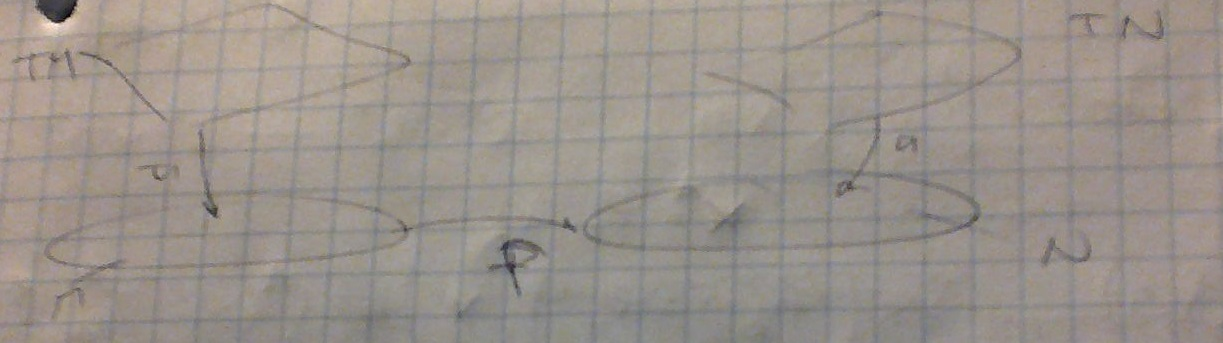
\includegraphics[width=0.5\textwidth]{TempPictures/TangentMap.jpg}
  \centering
\end{figure}

\begin{definition}[Tangent Map]
Is the map $\textrm{T}f := \textrm{d}f \; : \; TM \rightarrow TN$ such that:
\begin{displaymath}
\textrm{T}f \; : V_p \in T_pM \mapsto \big[ \big( f_*(p) \big) V \big] \in T_{f(p)}N
\end{displaymath}

\end{definition}

\begin{observation}
In differential geometry it's usual to give different name to objects that are essentially the same in order to emphasize some \emph{"flavour"}.
\\
In this case, we have:
\begin{itemize}
\item $\textrm{d}f(p)$ : " Differential of $f$" is the linear operator between $T_pM \rightarrow T_{f(p)}N$ for a fixed $p\in M$.

\item $f_*(p)\, V$ : " Push-Forward through $f$ of a tangent vector $V$"  is the image of $\textrm{d}f(p)$ on $V\in T_pM$.

\item $\textrm{T}f$ : " Tangent map of f" is the vector-bundle-morphism which act on every fiber like the differential operator.

\end{itemize}

\end{observation}


\subsection{Vector fields and natural references.}

\begin{notationfix}
The section of $TM$ are called \emph{vector fields} on the manifold $M$.
The reason is straightforward:
\\ Fixing a point in $TM$ is equivalent to pick a point in $M$ and a vector in $\mathbb{R}^n$, thus it represent a tangent vector of base point $p$.
\\ Known that a vector field could be easily seen as a map $V:M \rightarrow TM$ satisfying the section condition $ \pi \cdot V = \mathbb{1}_M$.
\end{notationfix}

\begin{notationfix}
The collection of all vector fields is a section spaces always carried on every differential manifold, it's often indicated with a particular notation:
	\begin{displaymath}
	 \Gamma(TM) = \mathfrak{X}(M)
	\end{displaymath}
\end{notationfix}	

In coordiante chart we may read off the components of the vector.
\\Consider a local chart $(U, \phi)$ over $p$ such that $\phi=(x^1, \ldots, x^n )$:

\begin{definition}[Natural Reference]
Sections  $(\partial_1, \ldots, \partial_n) \subset \mathfrak{X}(M)$ of $TM$, such that:
	\begin{displaymath}
		\partial_j (p) = \frac{\partial}{\partial_j} \big \vert_p \in T_pM
	\end{displaymath}
i.e. are the fields which associate to every point in $M$ a natural tangent vector (tangent to the coordinate curve).
\end{definition}

\begin{observation}
Provided an atlas on $M$ is defined $\forall X \in \mathfrak{X}(M)$ the decomposition:
	\begin{displaymath}
		X= \sum_{j=1}^n a^j(p) \partial_j(p)
	\end{displaymath}
Where the component are:
	\begin{equation}\label{eq: vector fields components}
		a^j(p) = \textrm{d}\phi_p \big( X(p)\big) \in C^\infty(U)
	\end{equation}
ans $U$ is a neighborhood of $p$.
\end{observation}

\begin{observation}
	Obviously a change in local chart induce a transformation in local reference.
	\\
	Consider a second chart $( \tilde{U}, \tilde{\phi}$ with $ U \cap \tilde{U} \neq \emptyset$.
	The change of natural basis on a fixed tangent space is easily extended on the whole natural reference:
	\begin{equation}\label{eq: controvariant basis}
		\tilde{\partial_h} = \sum_{k=1}^n \frac{\partial x^k}{\partial \tilde{x}^H} \partial_k
	\end{equation}
	From that follows $X= \sum_j a^j \partial_j = \sum_k \tilde{a^k} \tilde{\partial_k} $ i.e. the covariant change rule :
	\begin{displaymath}
		a^j = \sum_h \frac{\partial x^j}{\partial \tilde{x}^h} \tilde{a}^h
	\end{displaymath}
	is extended to the section.
\end{observation}	
	
\subsection{CoTangent Bundle}
\begin{notationfix}
\emph{Cotangent Bundle} is a specific name for the specialization of \ref{Def: Dual vector bundle} to the tangent spaces, i.e. is vector bundle on $M$ with total space $T^*M = \underset{p \in M}{\sqcup}T^*_p M  $ and usual projection $\pi$.
\end{notationfix}

\begin{observation}
This vector bundle is unique, by theorem \ref{Teo: Reconstruction Vector Bundle 1}, providing the following transition functions for a change of trivialization chart.
\begin{itemize}
\item[ ] Recalling that for all local chart $\varphi = (x^1, \ldots, x^n)$ are defined:
	\begin{itemize}
	\item[$\cdot$] $\dfrac{\partial}{\partial x^h} \big\vert_p \in T_p M$ = natural basis vector  in $T_p M \quad \forall p \in U$.\footnote{Depending on which equivalent presentation of the tangent space is taken into account these can be seen as the tangent vector to the coordinate curve or as a partial derivative operator on $C^\infty (U)$.}
	\item[$\cdot$] $\textrm{d}x^h \big \vert_p in T_p^*M$ = external derivative of the local chart calculated in $p$.
	\end{itemize}

	follows directly from definition of \emph{external derivative} that:
	\begin{displaymath}
	\textrm{d}x^j_P \big( \frac{\partial}{\partial x^h} \big \vert_p \big) = \frac{\partial x^j}{\partial x^h}(p) = \delta^j_{\, h}
	\end{displaymath}
	in other words $\{ \textrm{d}x^h_P \}$ are the \emph{natural dual basis} 1-forms.

\item[ ] Recalling also that taken two overlapping chart $(U_\alpha, \phi_\alpha)$ , $(U_\beta, \phi_\beta)$ on $M$, we have
	\begin{displaymath}
	\textrm{d}x^k_{\beta} \big \vert_p = \sum_h \frac{\partial x^k_{\beta}}{\partial c^h _\alpha}\textrm{d}x^h_\alpha \big \vert_p
	\end{displaymath}
	i.e. dual coordinate are \emph{covariant} \footnote{To compare to \eqref{eq: controvariant basis}, the controvariant relation of the natural basis.}.

\item[•] Chosing a standard trivialization on the cotangent bundle:
	\begin{displaymath}
	\chi_\alpha \big( \sum_j w_j \textrm{d}x^j_\alpha \big \vert_p \big) = (p, w^T)
	\end{displaymath}
	where $w^T \in \mathbb{R}^n$ is simply the transposition of row vector of 1-form components $( w_1, \ldots, w_n)$.	
	
\item[•] Follows that:
	\begin{displaymath}
		\chi_\alpha \circ \chi_\beta^{-1} \big( p, w^T \big) =
		\chi_\alpha \big( w_j \textrm{d}x^h_\beta \big \vert_p \big) =
		\chi_\alpha \big( \big[ w_j \frac{\partial x^j_\beta}{\partial x^{\, h}_\alpha}\big \vert_p		\textrm{d}x^h_\alpha \big \vert_p \big) =
		\big( p, \big[ \frac{\partial x_\beta}{\partial x_alpha}(p) \big]^T w^T \big)	
	\end{displaymath}
\end{itemize}
In conclusion:
\begin{equation}
 \big[ g_{\alpha \beta} \big]^\cdot_{\, \cdot} = \big[\frac{\partial x_\beta^\cdot}{\partial_\alpha^{\, \cdot} } \big] ^T
\end{equation}
are the transition map for the dual bundle \footnote{To confront with the tangent case in which $\big[ g_{\alpha \beta} \big]^\cdot_{\, \cdot} = \dfrac{\partial x^\cdot_\alpha}{\partial x^{\, \cdot}_\beta}$ .}.
\end{observation}

\begin{notationfix}
The cross section of the cotangent bundle are called \emph{1-forms} on $M$
\end{notationfix}

\begin{observation}
Is possible to review the concept of \emph{external derivative} in the language of tangent bundles and 1-forms \cite{abate}.
\\
$\forall f \in C^\infty(M)$ $\textrm{d}f$
 is the function $ \textrm{d}f : TM \rightarrow T \mathbb{R} $ such that:
	\begin{equation}
		\textrm{d} f \big( V_p \big) = V(f) \big \vert_p \qquad \forall V \in \mathfrak{X}(M)
	\end{equation}
\end{observation}

\begin{observation}
The dual natural reference is then provided by the external derivative of the local chart and they are the operator $\textrm{d} x^a (p) $ that returns the component of a vector fields seen in equation \eqref{eq: vector fields components} .
\end{observation}

\subsection{Tensor Bundle}
As last effort we can combine all the precedent definition to introduce the tensor bundle:

\begin{definition}[$(k,l)-$Tensor Bundle]
Is the unique vector bundle :
	\begin{displaymath}
		T^k_l M = \underbrace{T^*M \otimes \cdots \otimes T^*M}_{\textrm{k-times}} \otimes \underbrace{TM \otimes \cdots \otimes TM}_{\textrm{l-times}}
	\end{displaymath}
i.e. such that each fiber is in the form $E_p = T^k_l \big(T_p M) \big) $.	
\end{definition}

\begin{observation}
	Uniqueness follows from definition of $\times$ for vector bundles.
	\\
	Anyway the transition map for such bundle follows from the transformation of tensor components under change of local charts (see \cite{abate}).
\end{observation}

\begin{notationfix}
	The section of $T^k_l(M)$ are called \emph{tensor fields}.
\end{notationfix}

%-_-_-_-_-_-_-_-_-_-_-_-_-_-_-_-_-_-_-_-_-_-_-_-_-_-_-_-_-_-_-_-_-_-_-_-_-_-_-_-_-_-_-_-_-_-_-_-_-_-_-_-_-_-_-_
\subsection{Phase Space}

	\begin{notationfix}
In the context of Classical mechanics is customary to refer to the cotangent bundle $T^*Q$ over the smooth manifold  $Q $ - called \emph{Configuration Space}  - as \emph{Phase Space}.
	\end{notationfix}
	Since $TQ$ and $T^*Q$ are diffeomorphic , it might seem that there is no particular reason in treating this two spaces separately, but it is not so.
	There are certain geometrical objects that live naturally on $T^*Q$ , not on $TQ$.
	Of greatest interest in mathematical-physics are the Poincarè forms\cite{Fraenkel}.
	
	Consider a smooth manifold $Q$ and call $\Phase=T^*Q$ the corresponding cotangent bundle.
	\begin{definition}[Tautological (Poincarè) 1-form]
		Is the 1-form over $\Phase$:
		\begin{displaymath}
			\theta_0 \in \Gamma^\infty (T^*\Phase)
		\end{displaymath}
		such that the action on a generic point $ \omega_{\alpha_p} \in T_{\alpha_p}M$ ( in the fiber of $\alpha_p$, which in turn is a one-form on the fiber of $p\in Q$) is given by:
		\begin{displaymath}
			\theta_0 \big(\alpha_p \big): T_{\alpha_p}\Phase \rightarrow \Real \qquad : \; \omega_{\alpha_p} \mapsto \alpha_q \circ T \tau^*_Q \big( \omega_{\alpha_p} \big)
		\end{displaymath}
			\footnote{For a slightly different formulation see : \cite{fraenkel} \cite{fomm} \href{https://en.wikipedia.org/wiki/Tautological_one-form}{wiki}}
	\end{definition}
	\begin{figure}[h!]
   		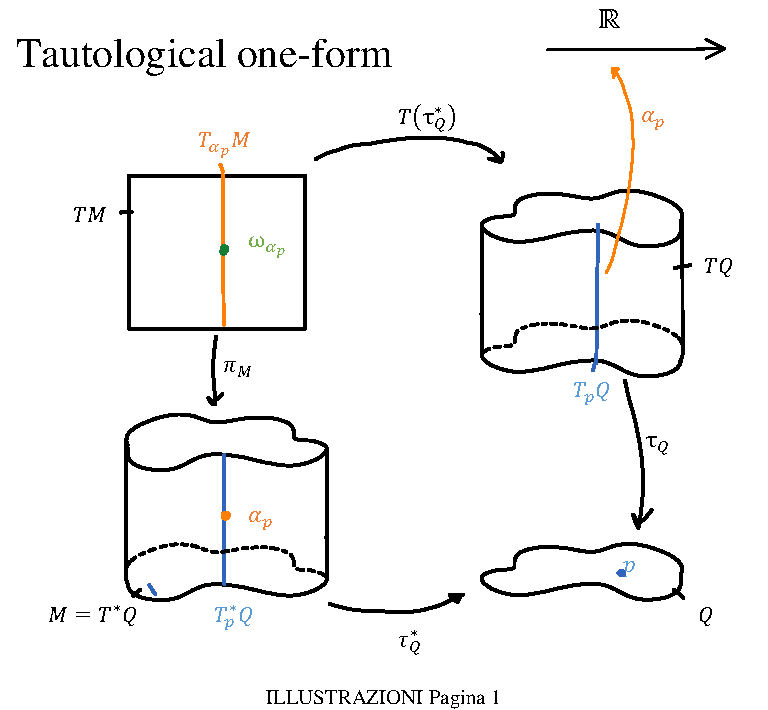
\includegraphics[width=0.5\textwidth]{Pictures/Tautological1Form} 
 		\caption{The definition of tautological 1-form is achieved exploiting the concept of \emph{Tangent map} and remembering that $\alpha_p: T_p \Phase \rightarrow \Phase$ is a linear functional.} 
  		\centering
	\end{figure}
		\begin{notationfix}
		Canonical coordinates are defined as a special set of coordinates on the cotangent bundle of a manifold. 
		They are usually written as a set of $(q^i,p_j)$ where ${q_i}$ are denoting the coordinates on the underlying manifold and the ${p_j}$ are denoting the conjugate momentum, which are decomposition of 1-forms in $T_p^*M$ on the dual natural basis $d q^J$ in the cotangent bundle at point $q$ in the manifold.
	\end{notationfix}
	
	\begin{proposition}[Coordinate Representation of $\theta_0$]
		In canonical coordinate the tautological one-form assumes the famous expression:
		\begin{displaymath}
			\theta_0 = \sum_{i=1}^n p_i d q^i
		\end{displaymath}
		(note that $d q^i$ is a 1-form on $T^*M$ calculated with respect to the coordinate on the bundle. Has not to be confused with the 1-natural form $d q^i \in T^*_p M$.)
	\end{proposition}
	\begin{proof}
		See \cite{fomm}[pag 179]
	\end{proof}
	
		\begin{definition}[Canonical (Poincarè)  symplectic form]
			Symplectic form:
			\begin{displaymath}
				\omega_0 \coloneqq -d \theta_0
			\end{displaymath}
			In canonical coordinates assumes the famous expression:
			\begin{displaymath}
				\omega_0 \coloneqq \sum_{i=1}^n d p_i \wedge d q^i
			\end{displaymath}
		\end{definition}
	
	\begin{proposition}[Canonical symplectic form]
			$\omega \coloneqq d \theta_0$ is a symplectic 2-form on $M$.
	\end{proposition}
	\begin{proof}
	 Theorem 3.2.10 \cite{fomm}
	\end{proof}
	
	\begin{proposition}[Canonical Coordinate Representation]
	
	\end{proposition}
	
		As a mathematical curiosity, we note that the cotangent bundle of any manifold is orientable. Indeed, it carries a symplectic structure and hence a volume element.
		
		\danger Repetita \\
		The claim is proved by the following definition:
					\begin{definition}[Canonical (Poincarè)  symplectic form]
						Symplectic form:
						\begin{displaymath}
							\omega_0 \coloneqq -d \theta_0
						\end{displaymath}
						In canonical coordinates assumes the famous expression:
						\begin{displaymath}
							\omega_0 \coloneqq \sum_{i=1}^n d q^i \wedge d p_i
						\end{displaymath}
					\end{definition}



\section{Higher-order tangent bundles}
	\begin{Warning}
	\href{https://en.wikipedia.org/wiki/Tangent_bundle}{wiki:Higher-order tangent bundles}\\
Since the tangent bundle $TM$ is itself a smooth manifold, the second-order tangent bundle can be defined via repeated application of the tangent bundle construction:

$$T^2 M = T(TM)$$
In general, the k-th order tangent bundle $T^k M$ can be defined recursively as $T(T^{k-1}M)$.

A smooth map $f : M \rightarrow N$ has an induced derivative, for which the tangent bundle is the appropriate domain and range $Df : TM \rightarrow TN$. 
Similarly, higher-order tangent bundles provide the domain and range for higher-order derivatives $D^k f : T^k M \mapsto T^k N$.

A distinct but related construction are the jet bundles on a manifold, which are bundles consisting of jets.
	\end{Warning}

\section{Jet Bundles}
The jet bundle is a certain construction that makes a new smooth fiber bundle out of a given smooth fiber bundle.

	The first step is to define the fiber of this new construction.
	Suppose M is an m-dimensional manifold and that (E, π, M) is a fiber bundle.
	
	Consider the set of all the local sections whose domain contains $p$
	\begin{displaymath}
		\Gamma^\infty (p) \coloneqq \big\{ \sigma \in \Gamma^\infty(E) \quad \big\vert\:  p \in \dom(\sigma)  \big\}
	\end{displaymath}
	two such section $\sigma, \eta \in \Gamma^\infty(p)$ have the \underline{same \emph{r-jet} at $p$} iff:
	\begin{displaymath}
		\left.\frac{\partial^{|I|} \sigma^{\alpha}}{\partial x^{I}}\right|_{p} = \left.\frac{\partial^{|I|} \eta^{\alpha}}{\partial x^{I}}\right|_{p}, \quad 0 \leq |I| \leq r.
	\end{displaymath}
	where $I={i_1, i_2, \ldots, i_m}$ is a \emph{Multi-index}.
	\begin{notationfix}
		\begin{displaymath}
			|I| := \sum_{i=1}^{m} I(i)
		\end{displaymath}
		\begin{displaymath}
			\frac{\partial^{|I|}}{\partial x^{I}} := \prod_{i=1}^{m} \left( \frac{\partial}{\partial x^{i}} \right)^{I(i)}
		\end{displaymath}
	\end{notationfix}
	
	We define the \emph{r-th Jet} as the equivalence class under this relation.
	\begin{notationfix} 
		r-jet with representative σ is denoted $j^r_p\sigma$ . 
		The integer r is also called the order of the jet, p is its source and σ(p) is its target.
	\end{notationfix}
	
	We define the jet fiber $J^r_p (E)$ on the point $p$ as the set of the equivalence classes:
	
	\begin{definition}[r-th Jet Bundle of $E$]
		The triple $(J^r(E), \pi_r, M)$	where:
		\begin{itemize}
			\item $J^r(E) \coloneqq \big\{j^r_p\sigma \quad \vert \; p\in M, \; \sigma \in \Gamma^\infty(p) \big\}$
			\item $\pi_r: J^r(E) \rightarrow M$ such that $j^{r}_{p}\sigma \mapsto p $
		\end{itemize}
	\end{definition}
	
	\begin{propostion}
		$ J^r(E) = (J^r(E), \pi_r, M)$ is a smooth bundle.
	\end{proposition}









%-_-_-_-_-_-_-_-_-_-_-_-_-_-_-_-_-_-_-_-_-_-_-_-_-_-_-_-_-_-_-_-_-_-_-_-_-_-_-_-_-_-_-_-_-_-_-_-_-_-_-_-_-_-_-_
\newpage
\section{Closing Thoughts}
\subsection{Prima stesura dell'introduzione}
In questo primo capitolo ci concederemo un po' di tempo per presentare i \emph{fibrati}, una famiglia di strutture algebriche di particolare importanza per la fisica-matematica moderna.

L'approccio che seguiremo è in un certo senso deduttivo.

Partiremo definendo la struttura, particolarmente astratta, di \emph{Fiber Bundle} sopra la categoria degli spazi topologici; sottolineando come questo rappresenti il setting più generale per rappresentare il concetto di campo nell'accezione originata dalla fisica ma senza tralasciare il fatto che la famiglia dei bundle costituisca una categoria concreta (costrutto) di per sè.

Nel paragrafo 2 arricchiremo questo oggetto astratto con una , così detta, \emph{G-Structure}. Una soppalcatura che va necessariamente fissata se si vuole disporre di un concetto di compatibilità tra trivializzazioni overlapping.

Nel terzo paragrafo si specializzerà la categoria su cui viene definito il fibrato a non essere semplicimente quella degli spazi topologici ma la sottocategoria delle varietà smooth \footnote{in realtà per quanto detto in questo capitolo dovrebbe essere valido per qualsiasi ordine di differenziabilità. (per quanto riguarda hausdorff e second countability?)}.
Questo passaggio porta con se la possibilità di esplorare il rapporto tra gli spazi tangenti delle due varietà( base e totale) che costituiscono il fibrato. Il mezzo per formalizzare questo rapporto saranno le operazioni di \emph{Lift} e \emph{Drop}, specializzazione a questo contesto delle note operazioni di \emph{Pull-Back} e \emph{Push-Forward} tra varietà.

Nel paragrafo 4 si porrà per la prima volta un vincolo sulla spazio fibra imponendo che esso sia dotato 
della struttura di spazio lineare.
Si parlerà quindi di \emph{Vector Bundle} 
\footnote{In what follows we only consider \emph{smooth} Vector Bundle.} 
in questo contesto meno generale ci porremo il problema di dare di stabilire in quali condizioni è possibile definire un fibrato su una varietà disponendo solo di una collezione di fibre omeomorfe.

Nel capitolo quinto verranno analizzati i \emph{Tangent Bundle} la più importante classe di fibrato vettoriale sulle varietà lisci.

(...)

Infine ci si chiederà come iterare la struttura di spazio tangente analizzando il rapporto tra i fibrati tangenti sulle due varietà costituente un generico bunle smooth.


\subsection{Eliminata}
Questioni di interesse personale che non ho aggiunto al capitolo per esigenze di tempo  in quanto non strettamente legati agli argomenti della tesi oppure da spostare secondo consiglio di CD:
\begin{itemize}


\item In letteratura si vede spesso riferirsi alla G-struttura del fibrato come \emph{Gauge Group}... Perchè?

\item La questione di chart vs trivialization è una riflessione fatta da me superflua per la tesi.. qua ho scritto quasi tutto ma sui miei appunti cartacei ho messo qualche schemino in più.. (quindi li ho scannerizzati e messi nel materiale della tesi!)

\item Approccio generale( nel senso di non limitarsi alle varietà riemmaniane) alle connessioni con il linguaggio dei fribrati\\ la formulazione precisa si fa molto efficacemente disponendo degli spazi doppio tangenti:
\\	specificare un unico lift
\\	trasporto parallelo
\\	curvatura

\item Teoremi di costruzione dei vector bundle aggregando insieme un po' di spazi vettoriali. La fonte principale è abate. Ma io ho riscritto tutto a pagine 9,10,11 degli appunti della tesi.
Non sono superflui, servono essenzialmente per dimostrare che TM e T*M sono dei vector bundle!

\item Si parla (per esempio sull'abate capitolo 3 ultimo paragrafo) dei fibrati principali dei riferimenti associati ad un fibrato vettoriale. Salto questo argomento perchè non serve per la tesi.

\item ho visto il fibrato come una tripla ma... immaginiamo di avere una varietà M, cose vuol dire "dare un fibrato su di essa?" il secondo teorema del capito sui fibrati vettoriali risponde un po' a questa questione
\\ inoltre... che vuol dire fissare un punto sul total space ? vuol dire scegliere una coppia $(p,v)$ previa la scelta di una trivializzazione.
\\ invece nei vettoriali equivale esattamente a dare la coppia $(e,v)$, la scelta  di una trivializzazione equivale invece ad una scelta di base in $F$ tale di decomporre il vettore $v$ in una n-pla.

\item Abate per definite il $\otimes$ di bundle passa per la definizione di fiber product set (vedi abate e appunti pag 12) .. io ho preferito passare direttamente alla def per i bundle.

\item riguardo alla tangent map il FOM appesantisce molto la notazione e i concetti... io sui miei fogli ho seguito un po' la sua strada ma mi sembra tutto superfluo... differenziale, push forward e tangent map sono in fondo la stessa cosa

\item la parte sul doppio tangent bundle come setting per la connessione la salto (magari la metto come parte nel capitolo due dove c'è la geometria riemmaniana o forse non lo metterò mai!).
\\ Si può però fare un accenno alla ricorsione del tangent bundle come fa qui: \href{http://en.wikipedia.org/wiki/Tangent_bundle#Higher-order_tangent_bundles}{Wiki Tangent Bundle}

\item la questione di rividere il dual tangent space come una varietà simplettica è da mettere nella parte sulla meccanica classica geometrica. in quanto, dice dappiaggi, è solo in questo contesto che si usa questa proprietà!

\item nel jurgen jost, capitolo sui fibrati, ci sono delle interessanti proposizioni sui fiber bundle su varietà riemmaniane, si afferma che in questo caso la G-Structure è garantita

\item ispirato da Fraenkel ho scritto sui miei appunti la dimostrazione che $TM$ e' una varieta' differenziale. In realtà la cosa è superflua se si sfrutta il teorema di ricostruzione del vector bundle.

\end{itemize}


\subsection{Possibile Estensioni}
Per capitoli
\begin{enumerate}
\item FB

\item GB

\item SB

\item VB
	\begin{itemize}
		 \item Considerazioni sul vector bundle.Che vuol dire in parole provere fissare un punto sul fibrato.
		 \item (da wiki VB) esempi: trivial bundle, moebius strip
		 \item (da wiki VB) accenno ai banach bundle
		 \item Nell'ottica della quantizzazione è necessario parlare  del bundle innerproduct
	\end{itemize}

\item TB
	\begin{itemize}
		 \item (da freed) osservazione pag4 > $g_{\beta \alpha} = \textrm{d} ( x_\beta \circ x_\alpha^{-1})$
		 \item (da fraenkel) $TM$ as set is a manifold.
		 \item (Abate pag 139) Tangent bundles as sub category, morhism = tangent map
		 \item (fraenkel e alt) $T^*M$ as a phase space and natural simplectic structure (dapp dice di presentare i concetti meccanici in un altro capitolo)
		 \item paragrafo di confronto di mappe tra tangent bundle,\\ tangent map vs pull/push vs differential operator \\ fiber derivative 
		 \item Tangent bundle over riemmanian manifold (pag 37-39 Jurgen Jost)
		 \item Vector bundle of p-form ( pag 40-41 Jurgen Jost)
	\end{itemize}

\item TTB
	\begin{itemize}
		 \item Presentazione del doppio tangente nello spirtito di wiki (wiki VB pag 4)
		 \item (Wiki VB) Vertical lift
		 \item (WIKI TTB)
	\end{itemize}
\end{enumerate}

\vspace{8mm}
Possibili fonti da considerare:
\begin{itemize}
	\item Xavier Gracia, FIBRE DERIVATIVES: SOME APPLICATIONS TO SINGULAR LAGRANGIANS 
	\item \url{http://www.math.toronto.edu/selick/mat1345/notes.pdf}{Link}
	\item Koszul, Lectures on fiber bundles, \url{http://www.math.tifr.res.in/~publ/ln/tifr20.pdf}{Link}
	\item jmf, Connections on principal fibre bundles \url{http://empg.maths.ed.ac.uk/Activities/GT/Lect1.pdf}{Link}
	\item \url{http://personal.maths.surrey.ac.uk/st/T.Bridges/GEOMETRIC-PHASE/Connections_intro.pdf}{ConnectionsIntro}
	\item \url{http://math.stanford.edu/~ralph/fiber.pdf}{Topology of Fiber Bundles}
	\item \url{https://www.ma.utexas.edu/users/dafr/M392C/Notes/FiberBundles.pdf}{Freed}
	\item \url{http://www.cjcaesar.ch/fribourg/docfrib/fibre_bundles/fibre_bundles.pdf}{michael laurent}
	\item \url{www1.maths.leeds.ac.uk/~ahubery/Fibre-Bundles.pdf}{Leeds, fiber bundle}
	\item Google in generale,, ovviamente c'e' tanto! \url{https://www.google.it/search?q=FibreBndls.pdf&ie=utf-8&oe=utf-8&rls=org.mozilla:en-US:unofficial&client=iceweasel-a&channel=sb&gws_rd=cr&ei=uQ-tVM_0DMKtygOBvoGwDA#rls=org.mozilla:en-US:unofficial&channel=sb&q=fibre+bundles}{goog}	
	\item Connection on fiber bundles \url{http://en.wikipedia.org/wiki/Connection_%28vector_bundle%29}{wiki}	
	
\end{itemize}

\subsection{TODO}
\begin{itemize}
\item Ricopiare dimostrazione \ref{Teo: Reconstruction Vector Bundle 2}

\item rifare tutte le illustrazioni con inkscape.
\end{itemize}

\subsection{Take away messages.}
	...
%-_-_-_-_-_-_-_-_-_-_-_-_-_-_-_-_-_-_-_-_-_-_-_-_-_-_-_-_-_-_-_-_-_-_-_-_-_-_-_-_-_-_-_-_-_-_-_-_-_-_-_-_-_-_-_


\begin{thebibliography}{100}
\bibitem{freed} Daniel S. Freed - Fiber Bundles and Vector Bundles -https://www.ma.utexas.edu/users/dafr/M392C/Notes/FiberBundles.pdf

\bibitem{abate} Marco Abate and Francesca Tovena - \emph{Geometria differenziale}.

\bibitem{fomm} Ralph Abraham and Jerrold E. Marsden -  \emph{Foundations of Mechanics}.

\bibitem{fraenkel} Theodore Frankel -  \emph{The geometry of Physics}.

\bibitem{advances} Benini, M. and Dappiaggi, C. in Advances in AQFT 1–49

\bibitem{primer} Benini, M., Dappiaggi, C. and Hack, T.-P. Quantum Field Theory on Curved Backgrounds — a Primer. Int. J. Mod. Phys. A 28, 1330023 (2013).

\end{thebibliography}






\end{document}